% !TEX TS-Program = pdflatex

\documentclass[12pt]{article}

\newcommand{\course}{MA440}

\usepackage{geometry}
\geometry{
    letterpaper,
    margin=0.8in,
    % left=0.8in,
    % top=0.8in,
    % headsep=\baselineskip,
    % textwidth=26pc,
    % marginparsep=2pc,
    % marginparwidth=12pc,
    % textheight=38\baselineskip,
    % headheight=2\baselineskip,
    % includemp,
    % reversemarginpar,
    % bindingoffset=1cm,
    twoside,
    asymmetric
}

\usepackage{amsmath}
% \usepackage{amsthm}

% \usepackage{libertine}  %%%%%The Linux Libertine font family
% \usepackage[libertine]{newtxmath}

\usepackage{comicneue}
% \usepackage{noto-serif}
\usepackage[default]{lato}
\usepackage{libertinust1math}

\usepackage{pifont,manfnt,bbding}

\usepackage[T1]{fontenc}
\usepackage[protrusion=true,expansion=true]{microtype}

\usepackage{datetime}
\newdateformat{mydate}{\monthname[\THEMONTH], \THEYEAR}

\newdateformat{lastupdated}
{\THEMONTH/\THEDAY/\THEYEAR}

\newdateformat{semester}{
  \ifthenelse{\THEMONTH=1}{Winter \THEYEAR}{
    \ifthenelse{\THEMONTH<6}{Spring \THEYEAR}{
      \ifthenelse{\THEMONTH>8}{Fall \THEYEAR}{
        Summer \THEYEAR
      }
    }
  }
}

\usepackage{titling}

\renewcommand{\sectionmark}[1]{ \markright{#1}{} }

\usepackage{fancyhdr}
\pagestyle{fancy}

\fancyhf{}
% \fancyhfoffset[L]{14pc}
\setlength{\headheight}{18.0pt}
\addtolength{\topmargin}{-6.0pt}

\renewcommand{\headrulewidth}{1pt}
% \renewcommand{\footrulewidth}{1pt}
\fancyhead[RE,LO]{\bf \course}
% \fancyhead[RO,LE]{\thepage}
\fancyhead[C]{\large\bf Topic \leftmark}
% \fancyfoot[RE, LO]{\raisebox{-10\baselineskip}{\semester{\thedate}}}
% \fancyfoot[RO, LE]{\raisebox{-10\baselineskip}{\hfill \sffamily \theauthor}\hspace{-1ex}}
% \fancyfoot[C]{\raisebox{-10\baselineskip}{\thepage}}
\fancyfoot[C]{\thepage}

% \usepackage{ifthen}
% \usepackage{xparse}
\usepackage{ifoddpage}

% \usepackage{eso-pic}

% \NewDocumentCommand{\addBG}{}{
%   \AddToShipoutPicture{
%     \AtTextLowerLeft{
%       \put(-1pc,\LenToUnit{-\baselineskip}){
%         \rule[0em]{1.5pt}{\dimexpr \textheight+2\baselineskip}
%       }
%     }
%   }
% }

\NewDocumentCommand{\newlecture}{}{
  \newpage
  \checkoddpage
  \ifoddpage
  \else
    \clearpage
    \thispagestyle{empty}
    % \ClearShipoutPictureBG
    \cleardoublepage
    \newpage
    % \addBG
  \fi
}

\usepackage{graphicx}
\usepackage[
  breaklinks = true,
  colorlinks = true,
  pdftitle = "MA440 Worksheets",
  pdfauthor = "Dr. Ye"
]{hyperref}
\usepackage{bookmark}
\usepackage{longtable}
\usepackage{calc}
\usepackage{booktabs}
\usepackage{array}
\usepackage{multirow}
\usepackage{multicol}
\usepackage{float}
\usepackage{colortbl}
\usepackage{pdflscape}
\usepackage{tabu}
\usepackage{tabularx}
\usepackage{threeparttable}
\usepackage{threeparttablex}
\usepackage[normalem]{ulem}
\usepackage{makecell}
\usepackage[svgnames]{xcolor}

% \usepackage{changepage}

% \newenvironment{fullwidth}{%
%   \begin{adjustwidth}{-14pc}{}%
%   \hsize=\linewidth%
% }{
%   \end{adjustwidth}
% }

\usepackage[inline]{enumitem}
\setenumerate{
	label=\textup{(\arabic*)},
	% afterlabel={\quad},
	%%vertical
	topsep=0pt,
	partopsep=0pt,
	% itemsep=6\baselineskip,
	parsep=2pt,
  % after=\vspace*{\dimexpr 6\baselineskip},
	% labelindent=0em,
	% itemindent = *,
	% itemindent=1ex,
	% wide,
	% itemjoin={\hspace{0.1\textwidth}},
	%%Horizontal
}
\setitemize{
	%%vertical
	topsep=0pt,
	partopsep=0pt,
	itemsep=0pt,
	parsep=0pt,
	%%Horizontal
	labelindent=0em,
	leftmargin =!,
	itemindent = 0pt,
	labelsep= 2pt,
	labelwidth=1em,
}
\setlist{topsep=0pt}

\SetEnumitemKey{sepno}{nosep, after=\vspace*{0pt}}

\SetEnumitemKey{twocol}{
itemsep = 1\itemsep,
parsep = 1\parsep,
before = \raggedcolumns\begin{multicols}{2},
after = \end{multicols}}

\SetEnumitemKey{threecol}{
itemsep = 1\itemsep,
parsep = 1\parsep,
before = \raggedcolumns\begin{multicols}{3},
after = \end{multicols}}

\SetEnumitemKey{fourcol}{
itemsep = 1\itemsep,
parsep = 1\parsep,
before = \raggedcolumns\begin{multicols}{4},
after = \end{multicols}}

\usepackage{tikz}
\usepackage{pgfplots}
\pgfplotsset{compat=newest}
\usepackage{pgfmath}
\usepackage{tikz-cd}
\usepackage{pgffor}
\usepackage{tkz-euclide}
\usepgfplotslibrary{fillbetween}
\usetikzlibrary{
    calc,
    angles,
    quotes,
    arrows.meta,
    math,
    backgrounds,
    pgfplots.statistics,
    matrix,
    patterns,
    shapes.geometric,
    spy,
    intersections,
    decorations.markings,
    decorations.pathmorphing,
    decorations.pathreplacing,
    decorations.shapes
}
\pgfdeclarelayer{ft}
\pgfdeclarelayer{bg}
\pgfsetlayers{bg,main,ft}
%%%%%%%%%%%%%%%%%%%%%%%%%%%%%%%%%%%%%%%%%%%%%%%%%%%%%%%%%%%%%%%%%%%%

%%%%%%%%%%%%%%%%% Setup the Coordinate System %%%%%%%%%%%%%%%%%%%%%%
\pgfplotsset{
    every axis/.style={
        %		 axis equal image,
        axis x line=middle,    % put the x axis in the middle
        axis y line=middle,    % put the y axis in the middle
        axis line style={-latex,very thick}, % arrows on the axis
        xlabel={$x$},          % default put x on x-axis
        ylabel={$y$},          % default put y on y-axis
        xlabel style = {font=\tiny, at={(xticklabel* cs:1)}, anchor=south},
        ylabel style = {font=\tiny, at={(yticklabel* cs:1)}, anchor=west},
        scaled ticks=true,
        x tick label style={font=\tiny, yshift=0.25ex, inner xsep=0pt},
        y tick label style={font=\tiny, xshift=0.25ex, inner ysep=0pt},
        grid style={black},
        % set layers=standard,
    }
}

%%%%%%%%%%%%%%% include files/Figure %%%%%%%%%%%%%%%%%%%%%%%%%%%%%%%%%
\usepackage{import}
% \usepackage{subfiles}
\usepackage{wrapfig}
%%%%%%%%%%%%%%%%%%%%%%%%%%%%%%%%%%%%%%%%%%%%%%%%%%%%%%%%%%%%%%%%%

%%%%%%%%%%%%%%%% Cancel common factors in Math %%%%%%%%%%%%%%%%%%%%
\usepackage[makeroom]{cancel}
%%%%%%%%%%%%%%%%%%%%%%%%%%%%%%%%%%%%%%%%%%%%%%%%%%%%%%%%%%%%%%%%%%%

%%%%%%%%%%%%%% Math mode without vertical spacing %%%%%%%%%%%%%%%%%
\makeatletter
\g@addto@macro\normalsize{%
    \setlength\abovedisplayskip{1pt plus 2pt minus 2pt}%
    \setlength\belowdisplayskip{1pt plus 2pt minus 2pt}%
    \setlength\abovedisplayshortskip{1pt plus 2pt minus 2pt}%
    \setlength\belowdisplayshortskip{1pt plus 2pt minus 2pt}%
}
\makeatother
%%%%%%%%%%%%%%%%%%%%%%%%%%%%%%%%%%%%%%%%%%%%%%%%%%%%%%%%%%%%%%%%

\newcommand{\ZZ}{\mathbf{Z}}
\newcommand{\RR}{\mathbf{R}}
\newcommand{\NN}{\mathbf{N}}
\newcommand{\QQ}{\mathbf{Q}}
\newcommand{\abs}[1]{\lvert #1\rvert}
\newcommand{\ii}{\mathbf{i}}
\newcommand{\parll}{ {\mathbin{\parallel}} }
\newcommand{\prll}{{\mathbin{\!/\mkern-5mu/\!}}}

\makeatletter
\renewcommand*\rel@kern[1]{\kern#1\dimexpr\macc@kerna}
\renewcommand*\widebar[1]{%
\begingroup
\def\mathaccent##1##2{%
\rel@kern{0.8}%
\overline{\rel@kern{-0.8}\macc@nucleus\rel@kern{0.2}}%
\rel@kern{-0.2}%
}%
\macc@depth\@ne
\let\math@bgroup\@empty \let\math@egroup\macc@set@skewchar
\mathsurround\z@ \frozen@everymath{\mathgroup\macc@group\relax}%
\macc@set@skewchar\relax
\let\mathaccentV\macc@nested@a
\macc@nested@a\relax111{#1}%
\endgroup
}
\renewcommand{\bar}{\widebar}
\newcommand*\centermath[1]{\omit\hfil~$\displaystyle#1$~\hfil\ignorespaces}
\newcommand{\cmc}{\centermath}
\newcommand*\ctc[1]{\omit\hfil\quad~ #1 ~\quad\hfil\ignorespaces}
\newcommand{\dfn}[1]{\textit{\textbf{#1}}}


%%%% Define Theorem Environment. Codes are modified from the Elegantbook class.

\usepackage[most]{tcolorbox}
\tcbuselibrary{theorems, hooks}

\newcommand{\proofname}{Proof}
\newcommand{\definitionname}{Definition}
\newcommand{\theoremname}{Theorem}
\newcommand{\lemmaname}{Lemma}
\newcommand{\propositionname}{Proposition}
\newcommand{\corollaryname}{Corollary}
\newcommand{\examplename}{Example}
\newcommand{\exercisename}{Exercise}
\newcommand{\remarkname}{Remark}
\newcommand{\solutionname}{Solution}

\newcommand{\thmcnt}{section}

\newlength{\normalparindent}
\setlength{\normalparindent}{\parindent}

\tcbset{
  common/.style={
    enhanced,
    breakable,
    % frame hidden,
    % opacityframe=.6,
    colback=white,
    coltitle=blue!90,
    grow to left by=1em,
    grow to right by=1em,
    left*=0pt,
    right*=0pt,
    boxrule=1pt,
    titlerule=0mm,
    % theorem hanging indent=0pt,
    arc=5pt,
    fonttitle=\upshape\bfseries,
    theorem style=plain,
    before upper app={\setlength{\parindent}{\normalparindent}},
    % adjusted title=left,
    % halign title=left,
    },
  defstyle/.style={
    % colback=green!10!white,
    colframe=green!80!black,
  },
  theostyle/.style={
    fontupper=\itshape,
    % colback=red!10!white,
    colframe=red!75!black
  },
  exmstyle/.style={
    frame hidden,
    % borderline east={1pt}{0pt}{blue!75!black},
    % overlay unbroken and last={%
    %     \draw[line width=1pt, blue!75!black, yshift=12pt] (frame.south east)   -- ++(0:-4cm);},
    colback=blue!5!white,
    % colframe=blue!75!black
    after app={\vspace*{8\baselineskip}}
  },
  ELEGANTtitle/.code n args={2}
    {
      \tcbset
        {
          title=
            {\csname #1name\endcsname~%
              \ifdef{\thetcbcounter}{\thetcbcounter}{}%
              \ifblank{#2}{}{\ (#2)}
            }
        }
    },
  % #1 is the command name of the theorem environment
  % #2 is the name of the theorem
  ELEGANTlabel/.code n args={2}
    {
      \ifblank{#2}
        {}{\tcbset{label={#1:#2}}}
    }
}


\NewDocumentCommand \ELEGANTnewtheorem { m m m O{}  }{
  \expandafter\ifblank\expandafter{#4}{
      \tcbset{
        new/usecnt/.style={}
      }
    }{
      \tcbset{
        new/usecnt/.style= {#4}
      }
    }
    \DeclareTColorBox[auto counter,number within=\thmcnt, usecnt]{#1}{ g o t\label g }{ % #1 is the command name of the theorem environment
    parskip, common, #3,
        % #3 is the thmstyle
        IfValueTF={##1}
          {ELEGANTtitle={#1}{##1}}
          {
            IfValueTF={##2}
            {ELEGANTtitle={#1}{##2}}
            {ELEGANTtitle={#1}{}}
          },
          % ##1 is the name of the theorem in tcolorbox format.
          % ##2 is the name of the theorem in amsthm format
        IfValueT={##4}
          { % ##4 is the label in tcolorbox format or the actual label in the command \label{}.
            IfBooleanTF={##3} % ##3 is value if \label{} is used.
              {ELEGANTlabel={##4}}
              {ELEGANTlabel={#2}{##4}}
          }
      }
    \DeclareTColorBox{#1*}{ g o }{
      parskip, common,#3,
        IfValueTF={##1}
          {ELEGANTtitle={#1}{##1}}
          {
            IfValueTF={##2}
            {ELEGANTtitle={#1}{##2}}
            {ELEGANTtitle={#1}{}}
          },
      }
  }

\ELEGANTnewtheorem{definition}{def}{defstyle}

\ELEGANTnewtheorem{theorem}{thm}{theostyle}[use counter from = definition]%

\ELEGANTnewtheorem{proposition}{prp}{theostyle}[use counter from = definition]%

\ELEGANTnewtheorem{lemma}{lem}{theostyle}[use counter from = definition]%

\ELEGANTnewtheorem{corollary}{cor}{theostyle}[use counter from = definition]%

\ELEGANTnewtheorem{example}{exm}{exmstyle}

\ELEGANTnewtheorem{solution}{}{exmstyle}[no counter]

\ELEGANTnewtheorem{proof}{}{exmstyle}[no counter]

\ELEGANTnewtheorem{remark}{}{defstyle}[no counter]

\newcounter{exer}[section]
\setcounter{exer}{0}
\renewcommand{\theexer}{\thesection.\arabic{exer}}

\newenvironment{exercise}[1][]{
  \refstepcounter{exer}
  \par\noindent\makebox[-3pt][r]{
    \footnotesize\color{red!90}\HandPencilLeft\quad}
    \comicneueangular
    \textbf{\color{blue!90}{\exercisename} \theexer ~~ #1}}{\vspace*{8\baselineskip}
    \par\ignorespacesafterend}



\title{\course~Worksheet}
\author{Dr. Ye}
\date{}

% \date{\semester{\today}}


\begin{document}
% \newgeometry{margin=1in}
% !TeX root =  main.tex

\let\cleardoublepage
% \clearpage

\thispagestyle{empty}%

	\vspace*{0.1\textheight}
	\begin{center}\leavevmode
		\normalfont
		{\HUGE\raggedright \textbf{\@title}\par}%
		\hrulefill\par
		{\huge\raggedleft {\@author}\par}%
		\vskip 1cm
		%    {\Large \@date\par}%
	\end{center}%

	\vfill

	\begin{center}\large
		Department of Mathematics and Computer Science\\

		Queensborough Community College - CUNY\\

		\the\year
	\end{center}

	\vspace*{2\baselineskip}

  \begin{center}
    {\color{blue} 
      Last updated on {\today}
    }
   \end{center}

   \newpage
% \restoregeometry

\newlecture
\addtocounter{page}{-2}
% !TeX root =  main.tex

\chapter{Functions}
\thispagestyle{chpg}

\section{Basic Concepts}
\begin{definition}
  A \textbf{relation} is a set of ordered pairs. The set of the first components of each ordered pair is called the \textbf{domain} and the set of the second components of each ordered pair is called the \textbf{range}.

  A \textbf{function} is a relation that assigns each element in the domain a unique element in the range.

  An arbitrary value in the domain is often represented by the lowercase letter $x$ which is called an \textbf{independent variable}.
  An arbitrary output is often represented by the lowercase letter $y$ which is called a \textbf{dependent variable}.
  
  % Each value in the domain is also known as an input value. Each value in the range is also known as an output value.
\end{definition}

\begin{example}
  Determine if the relation 
  \[\{(1,2),(2,4),(3,6),(4,8),(5,10)\}\]
  is a function. Find the domain and the range.
\end{example}

\begin{definition}
  If a function has $x$ as the independent variable and $y$ as the dependent variable, then we often say that $y$ is a function of $x$.
\end{definition}

\begin{example}
  Consider items and prices in a grocery store. Is price a function of item? Is item a function of price? 
\end{example}

\begin{definition}
  A function is often named by letters, such as $f$, $F$, $p$, or $q$. If $f$ is a function of $x$, then we denote it as $y=f(x)$ which is called the \textbf{function notation}. Here $f(x)$ is read as $f$ of $x$ or $f$ at $x$. The notation $f(x)$ represents the output of the function $f$ for a given input $x$.
\end{definition}
  
\begin{example}
  Use function notation to represent a function whose input is the name of a month and output is the number of days in that month.
\end{example}

\newpage


\begin{example}
  A function \(N=f(y)\) gives the number of police officers, \(N\), in a town in year \(y\). What does \(f(2005)=300\) represent?
\end{example}


\begin{example}
  Using a table to represent the days in the month as the function of month.
\end{example}

\begin{example}
  Consider the function $f(x)=x^2+3x-4$. Find the values of the following expressions.

\begin{enumerate}[fourcol]
  \item \(f(2)\)
  \item \(f(a)\)
  \item \(f(a+h)\)
  \item \(\dfrac{f(a+h)-f(a)}{h}\)
\end{enumerate}
\end{example}

\begin{example}
  Consider the function $f(x)=x^2-2x$. Find all $x$ values such that $f(x)=3$.
\end{example}

\newpage

\begin{example}
  Express the relationship defined by the function $2x-y-3=0$ as a function $y=l(x)$.
\end{example}


\begin{example}
  Does the equation \(x^2+y^2=1\) defines $y$ as a function $x$. If so, express the relationship as a function \(y=f(x)\). If not, under what extra condition does the function $y=f(x)$ exist? 
\end{example}


\begin{example}
  Consider the function $f(x)$ defined by a graph below.

  \begin{multicols}{2}
    \begin{enumerate}
      \item Find $f(-1)$. 
      \item Find all $x$ such that $f(x)=3$.
    \end{enumerate}
    \vfill

    \columnbreak
    
    \begin{tikzpicture}
      \begin{axis}[
      width=0.6\textwidth,
      xmin=-5,
      xmax=2,
      ymin=-2,
      ymax=5,
      xtick={-10,-9,...,10},
      ytick={-10,-9,...,10},
      ]
      \addplot[blue, line width=1.5pt, smooth,samples=100] {x^2+2*x} node[pos=0.2, right] {$y=f(x)$};
      \end{axis}
      \end{tikzpicture}

    % \begin{center}
    %   \includegraphics[scale=0.25]{figs/f(x)=x^2+2x.png}
    % \end{center}
  \end{multicols}
\end{example}
\vspace*{-12\baselineskip}

\newpage

\begin{definition}
  A function is a \textbf{one-to-one function} if each output value corresponds to exactly one input value.
\end{definition}

\begin{example}
  Is the area of a circle a function of its radius? If yes, is the function one-to-one?
\end{example}

\begin{howto}
  A graph is a function if very vertical line crosses the graph at most once. This method is known as the \textbf{vertical line test}.

A function is an one-to-one if very horizontal line crosses the graph at most once. This method is known as the \textbf{horizontal line test}.
\end{howto}

\begin{example}
  Determine if the graph defines a function. If so, is it a one-to-one function?
  \begin{center}
  \includegraphics[width=0.8\textwidth]{figs/cubic-line-circle.jpg}
  \end{center}
\end{example}

\newpage
\section*{Exercises}

\begin{exercise}
  Consider the function $f(x)=2x^2+x-3$. Find the values of the following expressions.

\begin{enumerate}[fourcol]
  \item \(f(-1)\)
  \item \(f(a)\)
  \item \(f(a+h)\)
  \item \(\dfrac{f(a+h)-f(a)}{h}\)
\end{enumerate}
\end{exercise}
\vspace*{2\baselineskip}

\begin{exercise}
  For the function $f(x)=-4x+5$, evaluate and simplify the difference quotient $\dfrac{f(x+h)-f(x)}{h}$.
\end{exercise}
\vspace*{2\baselineskip}

\begin{exercise}
  Consider the function $f(x)=-x^2-4x$. Find all $x$ values such that $f(x)=3$.
\end{exercise}

\newpage

\begin{exercise}
  Express the relationship defined by the function $3x-2y-6=0$ as a function $y=l(x)$.
\end{exercise}

\begin{exercise}
  If \(8x-y^3=0\), express \(y\) as a function of \(x\).

  Is $y$ a one-to-one function of $x$?
\end{exercise}


\begin{exercise}
  Consider the function $f(x)$ defined by a graph below.

  \begin{multicols}{2}
    \begin{enumerate}
      \item Find $f(1)$. 
      \item Find all $x$ such that $f(x)=3$.
    \end{enumerate}
    \vfill\mbox{}

    \columnbreak
   
    \begin{tikzpicture}
      \begin{axis}[
      width=0.6\textwidth,
      xmin=-2,
      xmax=5,
      ymin=-2,
      ymax=5,
      xtick={-10,-9,...,10},
      ytick={-10,-9,...,10},
      ]
      \addplot[blue, line width=1.5pt, smooth,samples=100] {-x^2+2*x+2} node[pos=0.7, right] {$y=f(x)$};
      \end{axis}
      \end{tikzpicture}

    % \begin{center}
    %   \includegraphics[scale=0.3]{figs/f(x)=-x^2+2x+2.png}
    % \end{center}
  \end{multicols}
\end{exercise}
\vspace{-10\baselineskip}


\newpage
\thispagestyle{fancy}

\section{Domains and Ranges}
\begin{howto}
The domain of a function $f$ consists of possible input values $x$. Or equivalently, the domain consists of all $x$ values except those that will make the function is undefined.

The range of a function $f$ consists of all possible output values $y$. Equivalently, the range consists of $y$ value such that equation $y=f(x)$ has a solution $x$. 
\end{howto}

\begin{example}
  Find the domain of the function $$f(x)=\dfrac{x+1}{2-x}.$$
\end{example}

\begin{example}
  Find the domain of the function
$$
f(x)=\sqrt{7-x}.
$$
\end{example}

\begin{definition}
  \textbf{Set-builder notation} is a method of specifying a set of elements that satisfy a certain condition. It takes the form $\{x|\text{ statement about x}\}$ which is read as, ``the set of all x such that the statement about x is true."
  
  \textbf{Interval notation} is a way of describing sets that include all real numbers between a lower limit that may or may not be included and an upper limit that may or may not be included. The endpoint values are listed between brackets or parentheses. A square bracket indicates inclusion in the set, and a parenthesis indicates exclusion from the set.
\end{definition}

\newpage

\begin{example}
  Find the domain of the function $f(x)=\dfrac{\sqrt{x+2}}{x-1}$. Write your answer in set-builder notation and interval notation.
\end{example}


\begin{example}
  Find the domain and range of the function $f$ whose graph is shown in Figure.

  \begin{tikzpicture}
    \begin{axis}[
    width=0.7\textwidth,
    xmin=-4,
    xmax=4,
    ymin=-2,
    ymax=10,
    xtick={-10,-9,...,10},
    ytick={-10,-9,...,10},
    ]
    \addplot[blue, line width=1.5pt, smooth,samples=100,domain=-3:2] {(-x^3+3*x)/2} node[pos=0.15,right] {$y=f(x)$};
    \addplot[mark=*, mark size=3pt] coordinates {(-3,9)};
    \addplot[mark=o, mark size=3pt] coordinates {(2,-1)};
    \end{axis}
    \end{tikzpicture}

  % \includegraphics[width=0.6\textwidth]{figs/FindDomainRangeCubic.png}
\end{example}
\vspace*{-8\baselineskip}

\begin{example}
  Find the domain and range of the function
  $$f(x)=\frac{2}{x+3}.$$
\end{example}

\newpage

\begin{example}
  Find the domain and range of the function
  $$f(x)=3\sqrt{x+2}.$$
\end{example}


\begin{example}
  Consider the piecewise function
  $$
  f(x)=\begin{cases}
    2x-3 & \text{if}\quad x\le -1\\
    -x^2 & \text{if}\quad -1<x< 1\\
    -2x+4 & \text{if}\quad 1\le x.
  \end{cases}
  $$
  \begin{enumerate}[threecol]
    \item Sketch the graph
    \item Find $f(-4)$
    \item Find $f(2)$
  \end{enumerate}
\end{example}

\newpage

\section*{Exercises}

\begin{exercise}
  Find the domain of the function\\
  \begin{enumerate*}
    \item  $f(x)=\dfrac{1+4x}{2x-1}$ 
    \item  $f(x)=\sqrt{5+2x}$
    \item  $f(x)=\dfrac{\sqrt{x+1}}{x-1}$
    \item $f(x)=\dfrac{x-2}{x^2+7x-44}$
  \end{enumerate*}
\end{exercise}
\vspace*{\stretch{5}}

\begin{exercise}
  Estimate the domain and range for the function defined by the graph. Write your answer in interval notation.\\
  \includegraphics[width=0.6\textwidth]{figs/CNX_Precalc_Figure_01_02_010.jpg}
\end{exercise}
\vspace*{-5\baselineskip}

\newpage

\begin{exercise}
  Find the domain and range of each of the following functions. Write your answer in set-builder notation and interval notation.
  \begin{enumerate}[twocol]
    \item $f(x)=\frac{3}{x-2}$
    \item $f(x)=-2\sqrt{x+4}$
  \end{enumerate}
\end{exercise}

\begin{exercise}
  Consider the piecewise function
  $$f(x)=\begin{cases}
    -2x+5 & \text{if}\quad x< -2\\
    x^2-1 & \text{if}\quad -2\le x\le 2\\
    2x-3 & \text{if}\quad 2< x.
  \end{cases}$$
  \begin{enumerate}[threecol]
    \item Sketch the graph
    \item Find $f(-4)$
    \item Find $f(2)$
  \end{enumerate}
\end{exercise}

\newpage

\section{Rates of Change and Behavior of Graphs}

\begin{definition}[Rate of Change]
  The average rate of change of $f$ over an interval $[a,b]$ is defined as
  $$\text{Average Rate Of Change}=\dfrac{f(b)-f(a)}{b-a}.$$
  The average rate of change is the same as the slope of secant line passing through $(a, f(a))$ and $(b, f(b))$.
  
  By taking $x=a$ and $h=b-a$, the average of rate of change is the same the difference quotient of a function $f$ which is defined as
  $$\text{Difference Quotient}=\dfrac{f(x+h)-f(x)}{h}.$$
\end{definition}

\begin{example}
  After picking up a friend who lives 10 miles away, Anna records her distance from home over time. The values are shown in Table. Find her average speed over the first 6 hours.
\begin{center}
  \begin{tabular}{l*{8}{c}}
    $t$ (hours) & 0 & 1 & 2 & 3 & 4 & 5 & 6 & 7\\
    $D(t)$ (miles) & 10 & 55 & 90 & 153 & 214 & 240 & 292 & 300
  \end{tabular}
\end{center}
\end{example}

\begin{example}
  Find the average rate of change of $f(x)=x^2-\dfrac{1}{x}$ over the interval $[2, 4]$.
\end{example}

\newpage

\begin{example}
  Find the average rate of change of  $g(t)=t^2+3t+1$ on the interval  $[0,a]$. The answer will be an expression involving $a$.
\end{example}



\begin{definition}[Increasing and Decreasing]
  A function $f$ is \textbf{increasing} over an interval $(a, b)$ if $f(x_2)>f(x_1)$ for any $x_1<x_2$ in $(a, b)$. Equivalently, $f$ is increasing over $(a, b)$ if  the average rate of change is positive over any subinterval $(x_1, x_2)$ of $(a, b)$.
  
  A function $f$ is \textbf{decreasing} over an interval $(a, b)$ if $f(x_2)<f(x_1)$ for any $x_1<x_2$ in $(a, b)$. Equivalently, $f$ is decreasing over $(a, b)$ if  the average rate of change is negative over any subinterval $(x_1, x_2)$ of $(a, b)$.

  \begin{center}
    \includegraphics[width=0.6\textwidth]{figs/CNX_Precalc_Figure_01_03_004.jpg}
  \end{center}
\end{definition}

\newpage

\begin{definition}[Local Maxima and Minima]
  A function \(f\) has a \textbf{local maximum} at \(x=c\) if $f(c)\ge f(x)$ for any $x$ in a small interval containing $c$. A small interval containing $c$ is also known as a small \text{neighborhood} of $c$.

  A function \(f\) has a \textbf{local minimum} at \(x=c\) if $f(c)\le f(x)$ for any $x$ in a small interval containing $c$.
\end{definition}

\begin{howto}
  A function $f$ has a local maximum at $x=c$ if it changes from increasing to decreasing at $c$ in a neighborhood of $c$.
  
  A function $f$ has a local minimum at $x=c$ if it changes from decreasing to increasing at $c$ in a neighborhood of $c$.
\end{howto}



\begin{example}
  Find the interval of increasing and the interval of decreasing, and the local maxima and local minima of the function $f$ defined by the following graph.

  \begin{tikzpicture}
    \begin{axis}[
    xmin=-3,
    xmax=3,
    ymin=-3,
    ymax=3,
    xtick={-10,-9,...,10},
    ytick={-10,-9,...,10},
    ]
    \addplot[latex-latex, blue, line width=1.5pt, smooth,samples=100,domain=-2:2] {x^3-3*x} node[pos=0.4, right] {$y=f(x)$};
    \end{axis}
  \end{tikzpicture}

  % \begin{center}
  %   \raggedright\includegraphics[width=0.5\textwidth]{figs/x^3-3x.png}
  % \end{center}
\end{example}

% \vspace*{-0.1\textheight}
% \newpage

\begin{definition}[Absolute Maxima and Minima]
  The \textbf{absolute maximum} of $f$ at \(x=c\) is \(f(c)\) where \(f(c)\ge f(x)\) for all \(x\) in the domain of \(f\).
  
  The \textbf{absolute minimum} of $f$ at \(x=c\) is \(f(c)\) where \(f(c)\le f(x)\) for all \(x\) in the domain of \(f\).
\end{definition}

\begin{example}
  Finding the absolute maximum and minimum of the function $f$ defined by the following graph.
  
  \begin{tikzpicture}
    \begin{axis}[
    % width=0.6\textwidth,
    xmin=-4,
    xmax=3,
    ymin=-3,
    ymax=4,
    xtick={-10,-9,...,10},
    ytick={-10,-9,...,10},
    ]
    \addplot[blue, line width=1.5pt, smooth,samples=100,domain=-3:1.5] {(-x^3+3*x-6)/4} node[pos=0.3, right] {$y=f(x)$};
    \addplot[mark=*, mark size=3pt] coordinates {(-3,3)};
    \addplot[mark=o, mark size=3pt] coordinates {(1.5,-1.21875)};
    \end{axis}
    \end{tikzpicture}

  % \begin{center}
  %   \raggedright\includegraphics[width=0.5\textwidth]{figs/(-x^3+3x-6)divby4.png}
  % \end{center}
\end{example}

\newpage
\section*{Exercises}

\begin{exercise}
  The electrostatic force  $F$, measured in newtons, between two charged particles can be related to the distance between the particles  $d$, in centimeters, by the formula  $F(d)=\dfrac{2}{d^2}$. Find the average rate of change of force if the distance between the particles is increased from 2 cm to 6 cm.
\end{exercise}

\begin{exercise}
  Find the average rate of change of $f(x)=x^2+2x-8$ on the interval $[5,a]$.
\end{exercise}

\begin{exercise}
  Find the interval of increasing and the interval of decreasing, and the local maxima and local minima of the function $f$ defined by the following graph.

  \begin{tikzpicture}
    \begin{axis}[
    xmin=-3,
    xmax=8,
    ymin=-8,
    ymax=3,
    xtick={-10,-9,...,10},
    ytick={-10,-9,...,10},
    ]
    \addplot[latex-latex, blue, line width=1.5pt, smooth,samples=100,domain=-2.8:7.8] {(x^3-6*x^2-15*x+16)/12} node[pos=0.4, right] {$y=f(x)$};
    \end{axis}
    \end{tikzpicture}
  % \begin{center}
  %   \raggedright\includegraphics[width=0.5\textwidth]{figs/(xcube-6xsq-15x+16)divby12.png}
  % \end{center}
\end{exercise}
\vspace{-12\baselineskip}

\newpage

\begin{exercise}
  Finding the absolute maximum and minimum of the function $f$ defined by the following graph.
  
  \begin{tikzpicture}
    \begin{axis}[
    width=0.6\textwidth,
    xmin=-3,
    xmax=4,
    ymin=-3,
    ymax=4,
    xtick={-10,-9,...,10},
    ytick={-10,-9,...,10},
    ]
    \addplot[blue, line width=1.5pt, smooth,samples=100,domain=-1.5:3] {(-x^3+3*x+10)/4} node[pos=0.6, right] {$y=f(x)$};
    \addplot[mark=*, mark size=3pt] coordinates {(3,-2)};
    \addplot[mark=o, mark size=3pt] coordinates {(-1.5,2.25)};
    \end{axis}
    \end{tikzpicture}

  % \begin{center}
  %   \raggedright\includegraphics[width=0.5\textwidth]{figs/(-x^3+3x+10)divby4.png}
  % \end{center}
\end{exercise}
\vspace*{-0.4\textheight}

\begin{exercise}
  Find the interval of increasing and the interval of decreasing, and the local maxima and local minima of the function $f(x)=x^3-6x^2-15x+20$ using its graph.
  %f\left(x\right)=2x^{3}-3x^{2}-12x+7
\end{exercise}

\newpage

\section{Combination and Composition of Functions}

\begin{definition}[Algebraic Operations of Functions]
  Let \(f\) and \(g\) be two functions with domains $A$ and $B$ respectively. We define the linear combination, product, and quotient functions as follows.
  \begin{center}
    \begin{tabular}{rcl}
      Linear combination: & $(af+bg)(x)=af(x)+bg(x)$ & with the domain $A\cap B$.\\
      Product: & $(fg)(x)=f(x)g(x)$ & with the domain: $A\cap B$.\\
      Quotient: & $\left(\dfrac{f}{g}\right)(x)=\dfrac{f(x)}{g(x)}$ & with the domain: $A\cap B\cap \{x\mid g(x)\neq 0\}$.
    \end{tabular}
  \end{center}
  
\end{definition}

\begin{example}
  Consider the functions \(f(x)=x-1\) and \(g(x)=x^2-1\). Find and simplify the functions \((g-f)(x)\) and \(\left(\dfrac{g}{f}\right)(x)\), and their domains.
\end{example}

\begin{definition}[Composition of functions]
  Let \(f\) and \(g\) be two functions with domains $A$ and $B$ respectively. The \textbf{composite function} $f\circ g$ (also called the
  composition of $f$ and $g$) is defined as
  \[(f\circ g)(x)=f(g(x))\qquad \text{with the domain:}\quad B\cap \{x\mid g(x)\in A\}.\]
\noindent
  We read the left-hand side as ``\(f\) composed with \(g\) at \(x\),'' and the right-hand side as ``\(f\) of \(g\) of \(x\).''
\end{definition}

\begin{example}
  Consider the functions \(f(x)=\sqrt{x-2}\) and \(g(x)=x^2+1\). 
  \begin{enumerate}
    \item Find and simplify the functions \((f\circ g)(x)\) and \((g\circ f))(x)\).  Are they the same function?
    \item Find the domains of $f\circ g$ and $g\circ f$. Are they the same?
  \end{enumerate}
\end{example}

\newpage

\begin{example}
  Consider $f(t)=t^2-4t$ and $h(x)=\sqrt{x+3}$. Evaluate\\ 
  \begin{enumerate*}
    \item $\dfrac{f(1)}{g(1)}$
    \item $h(f(-1))$
    \item $(f\circ h)(-1))$
    \item $(f-h)(-1)$
  \end{enumerate*}
\end{example}

\vspace*{2\baselineskip}

\begin{example}
  Using the graphs to evaluate the given functions.
  \begin{multicols}{2}
    \begin{enumerate}
      \item $(f+g)(1)$
      \item $(fg)(1)$
      \item $\left(\dfrac{f}{g}\right)(1)$
      \item $(g\circ f)(-3)$
      \item $f(g(0))$
      % \vfill\mbox{}
    \end{enumerate}
    \columnbreak
    \begin{tikzpicture}
      \begin{axis}[
        width=0.65\textwidth,
      xmin=-4,
      xmax=5,
      ymin=-4,
      ymax=5,
      xtick={-10,-9,...,10},
      ytick={-10,-9,...,10},]
      \addplot[blue, line width=1.5pt, smooth,samples=100] {-(x-2)^2+3} node[pos=0.85, right] {$y=g(x)$};
      \addplot[red, line width=1.5pt, smooth,samples=100] {(x+1)^2-2} node[pos=0.2, right] {$y=f(x)$};
      \end{axis}
      \end{tikzpicture}

    % \includegraphics[width=0.45\textwidth]{figs/twoquadratics.png}
  \end{multicols}
\end{example}
\vspace*{-0.1\textheight}

\begin{example}
  Consider the function $h(x)=\sqrt{x^2+1}$. Find two functions $f$ and $g$ so that $h(x)=f(g(x))$.
\end{example}

\newpage

\section*{Exercises}

\begin{exercise}
  Consider the functions \(f(x)=x^2-1\) and \(g(x)=x+1\). 
  \begin{enumerate}
    \item Find the function \((f-g)(x)\) and its domain.
    \item Find the function \((fg)(x)\) and its domain.
    \item Find \(\left(\dfrac{f}{g}\right)(x)\) and its domain.
    \item Find \((2f-3g)(1)\).
    \item Find \(2fg-\left(\dfrac{3g}{f}\right)(1)\).
  \end{enumerate}
\end{exercise}

\begin{exercise}
  Consider the functions $f(x)=\dfrac{1}{x-2}$ and $g(x)=\sqrt{x+4}$.

\begin{enumerate}
  \item Find $f\circ g$ and its domain.
  \item Find $(g\circ f)(3)$.
\end{enumerate}
\end{exercise}

\newpage

\begin{exercise}
    Using the graphs to evaluate the given functions.
    \begin{multicols}{2}
      \begin{enumerate}
        \item $(f-g)(1)$
        \item $(fg)(0)$
        \item $\left(\dfrac{f}{g}\right)(0)$
        \item $(f\circ g)(2)$
        \item $g(f(0))$
      \end{enumerate}

      \columnbreak

      \begin{tikzpicture}
        \begin{axis}[
          width=0.65\textwidth,
        xmin=-3,
        xmax=4,
        ymin=-3,
        ymax=4,
        xtick={-10,-9,...,10},
        ytick={-10,-9,...,10},]
        \addplot[blue, line width=1.5pt, smooth,samples=100] {-2*x^2+3} node[pos=0.6, above right] {$y=f(x)$};
        \addplot[red, line width=1.5pt, smooth,samples=100] {(x-1)^2-2} node[pos=0.6, above left] {$y=g(x)$};
        \end{axis}
        \end{tikzpicture}

      % \includegraphics[width=0.5\textwidth]{figs/two-quadratics-exr.png}
    \end{multicols}
\end{exercise}
\vspace*{-0.2\textheight}

\begin{exercise}
  Consider the function $h(x)=\sqrt[3]{2x-1}$. Find two functions $f$ and $g$ so that $h(x)=f(g(x))$.
\end{exercise}

\newpage

\section{Transformations}

\begin{definition}
  A function $y=g(x)$ that is obtained by substituting $x$ by $Bx-C$ and substituting $y$ by $Ay-D$, where $AB\ne 0$, from a function $y=f(x)$, is called a transformation of $f$.
  
  \begin{enumerate}
    \item If $A=B=1$ and $C=0$, $g$ is called a vertical shift of $f$ by $C$ units.
    \item If $A=B=1$ and $D=0$, $g$ is called a horizontal shift of $f$ by $D$ units.
    \item If $A=1$, $B=-1$ and $C=D=0$, $g$ is called a horizontal reflection or a reflection along the $y$-axis of $f$.
    \item If $A=-1$, $B=1$ and $C=D=0$, $g$ is called a vertical reflection or a reflection along the $y$-axis of $f$.
    \item If $A=1$ and $C=D=0$, $g$ is called a horizontal stretch or compression of $f$ by a factor $\dfrac{1}{B}$ if $0<B<1$ or $B>1$ respectively.
    \item If $B=1$ and $C=D=0$, $g$ is called a vertical stretch or compression of $f$ by a factor $\dfrac{1}{A}$ if $0<A<1$ or $A>1$ respectively.
  \end{enumerate}
\end{definition}


\begin{example}
  Consider the functions $f(x)=x^2$, $g(x)=x^2-1$ and $h(x)=x^2+2$.
  \begin{enumerate}
    \item Describe how to get the graph of $g$ from the graph of $f$.
    \vspace*{3\baselineskip}
    \item Describe how to get the graph of $h$ from the graph of $f$.
    \vspace*{3\baselineskip}
    \item Describe how to get the graph of $f$ from the graph of $h$.
    \vspace*{3\baselineskip}
    \item Describe how to get the graph of $h$ from the graph of $g$.
    \vspace*{3\baselineskip}
  \end{enumerate}
\end{example}

\begin{example}
  Consider the functions $f(x)=x^2$, $g(x)=(x+1)^2$ and $h(x)=(x-2)^2$.
  \begin{enumerate}
    \item Describe how to get the graph of $g$ from the graph of $f$.
    \vspace*{3\baselineskip}
    \item Describe how to get the graph of $h$ from the graph of $f$.
    \vspace*{3\baselineskip}
    \item Describe how to get the graph of $f$ from the graph of $h$.
    \vspace*{3\baselineskip}
    \item Describe how to get the graph of $h$ from the graph of $g$.
    \vspace*{3\baselineskip}
  \end{enumerate}
\end{example}

\newpage

\begin{example}
  Sketch the graph of \(f(x)=|x|\) and then use the graph to sketch the graph of \(h(x)=f(x+2)-1\). 
\end{example}

\begin{example}
  The function $y=g(x)$ shown in the picture is a shift of the square root function $y=\sqrt{x}$. Find $g(x)$.\\

  \begin{tikzpicture}[scale=1.2]
    \begin{axis}[
    xmin=-2,
    xmax=2,
    ymin=-2,
    ymax=2,
    xtick={-5,-4,...,5},
    ytick={-5,-4,...,5},]
    \addplot[blue, line width=1.5pt, smooth,samples=100,domain=-1:2] {sqrt(x+1)-1} node[pos=0.7, above left] {$y=g(x)$};
    \end{axis}
    \end{tikzpicture}
\end{example}
\vspace*{-0.4\textheight}

\newpage

\begin{example}
  Reflect the graph of \(f(x)=|x-1|\)\\
  \begin{enumerate*}
    \item first vertically,
    \item then horizontally.\hfill\mbox{}
  \end{enumerate*}

Denote the new function by $y=g(x)$. Find $g(x)$.
\end{example}

\begin{example}
  A common model for learning has an equation similar to \(k(t)=-2^{-t}+1\), where \(k\) is the percentage of mastery that can be achieved after \(t\) practice sessions, and $t>0$. The function $k$ is a transformation of a part of the function \(f(t)=2^t\) shown below. Sketch the graph of \(k(t)\).\\
  \begin{tikzpicture}
    \begin{axis}[
      width=0.75\textwidth,
    xmin=-5,
    xmax=5,
    ymin=-5,
    ymax=5,
    xlabel={$t$},
    ylabel={$k(t)$},
    xtick={-10,-9,...,10},
    ytick={-10,-9,...,10},]
    \addplot[blue, line width=1.5pt, smooth,samples=100,domain=-5:3] {2^x} node[pos=0.9, right] {$y=f(x)$};
    \addplot[mark=*] coordinates {(-2, 0.25)} node[above left] {$(-2,\frac14)$};
    \addplot[mark=*] coordinates {(-1, 0.5)} node[above left] {$(-1,\frac12)$};
    \addplot[mark=*] coordinates {(0, 1)};
    \addplot[mark=*] coordinates {(1, 2)} node[below right] {$(1,2)$};
    \end{axis}
    \end{tikzpicture}

% \includegraphics[width=0.5\textwidth]{figs/learningmodel.png}
\end{example}
\vspace*{-0.3\textheight}



\begin{example}
  The point $(9, -15)$ is on the graph of $y=f(x)$. Find a point on the graph of $g(x)=\dfrac{1}{3}f(x)$.
\end{example}
\vspace*{-0.3\textheight}

\newpage
\begin{example}
  The function $y=g(x)$ given in the following graph can be obtained from $f(x)=x^2$ by a combination of shifting, reflecting, and stretching. Describe the transformation and find an equation of $g$.\\
  \begin{tikzpicture}[scale=1.2]
    \begin{axis}[
    xmin=-3,
    xmax=5,
    ymin=-3,
    ymax=5,
    xtick={-10,-9,...,10},
    ytick={-6,-5,...,6},]
    \addplot[blue, line width=1.5pt, smooth,samples=100,domain=-1:3] {-2*(x-1)^2+4} node[pos=0.5, right] {$y=g(x)$};
    \end{axis}
    \end{tikzpicture}

  % \includegraphics[width=0.5\textwidth]{figs/transformationquadratic.png}
\end{example}
\vspace*{-0.1\textheight}

\begin{example}
  The function $y=f(x)$ has two $x$-intercepts $(-2, 0)$ and $(4, 0)$. Determine if the function $g(x)=f(2x)$ has any $x$-intercepts. If so, find them. Otherwise explain why it has no $x$-intercept.
\end{example}

\begin{example}
  Describe how to get the graph of the function $g(x)=4x^2$ from the graph of the function $f(x)$.
\end{example}
\newpage

\begin{example}
  Using the graph of the function $y=f(x)$ given below to sketch the graph of the function $g(x)=-2f(3x-6)+4$.\\
  \begin{tikzpicture}[scale=1.2]
    \begin{axis}[
    xmin=-3,
    xmax=3,
    ymin=-2,
    ymax=4,
    xtick={-10,-9,...,10},
    ytick={-6,-5,...,6},]
    \addplot[blue, line width=1.5pt, smooth,samples=100,domain=-2:2] {-abs(x)+2} node[pos=0.5, above right] {$y=f(x)$};
    \end{axis}
    \end{tikzpicture}

  % \includegraphics[width=0.5\textwidth]{figs/-abs(x)+2.png}
\end{example}

\newpage

\begin{example}
Sketch the graph of the function $g(x)=2\sqrt{3x-1}-4$ by a sequence of transformation applied on the graph of $f(x)=\sqrt{x}$.  
\end{example}

\begin{example}
  Find an equation of the function $y=g(x)$ whose graph is obtained from $f(x)=\sqrt{x}$ by the following transformations in the given order.
  \begin{enumerate}
    \item stretch vertically by a factor of 2
    \item shift downward 2 units
    \item shift 3 units to the left
    \item stretch vertically by a factor $\dfrac{1}{2}$.
  \end{enumerate}
\end{example}

\newpage

\begin{definition}
  A function is called an \textbf{even function} if $f(-x)=f(x)$ for $x$ in the domain of $f$.
  
  A function is called an \textbf{odd function} if $f(-x)=-f(x)$ for $x$ in the domain of $f$.
\end{definition}

\begin{remark}
  The graph of an even function is symmetric about $y$-axis.

  The graph of an odd function is symmetric about the origin. This symmetry is known as a rotation symmetry.
\end{remark}

\begin{example}
  Group the functions according to even, odd, or other.\\
  \begin{enumerate*}
    \item $f(x)=x^2-1$
    \item $g(x)=|x-1|$
    \item $h(x)=x^3-2x$
    \item $k(x)=\dfrac{1}{x^2}$.
  \end{enumerate*}
\end{example}


\newpage

\section*{Exercises}

\begin{exercise}
    Consider the functions $f(x)=x^2$, $g(x)=(x+1)^2-2$ and $h(x)=(x-2)^2+1$.
    \begin{enumerate}
      \item Describe how to get the graph of $g$ from the graph of $f$.
      \item Describe how to get the graph of $h$ from the graph of $g$.
    \end{enumerate}
\end{exercise}

\begin{exercise}
    Determine if the function is even, odd, or neither.\\
    \begin{enumerate*}
      \item $f(x)=1-x^2$.
      \item $g(x)=\sqrt[3]{-x}$.
      \item $g(x)=x^4-x^3$.
      \hfill\mbox{}
    \end{enumerate*}  
\end{exercise}

\newpage

\begin{exercise}
  Sketch the graph of the function $g(x)=2|3x-6| + 4$ by a sequence of transformation applied on the graph of $f(x)=|x|$.  
\end{exercise}

\begin{exercise}
  Find an equation of the function $y=g(x)$ whose graph is obtained from $f(x)=\sqrt[3]{x}$ by the following transformations in the given order.
  \begin{enumerate}
    \item Compress vertically by a factor of $\dfrac{1}{2}$.
    \item Reflect vertically.
    \item shift downward 2 units.
    \item Compress horizontal by a factor $2$.
    \item Shift 3 units to the right.
  \end{enumerate}
\end{exercise}

\newpage

\section{Inverse Functions}

\begin{definition}
  Let $y=f(x)$ be a one-to-one function with the domain $A$. A function \(f^{-1}(x)\) is an \textbf{inverse function} of \(f\) if \(f^{-1}(f(x))=x\) for all \(x\) in $A$.

The notation \(f^{-1}\) is read “\(f\) inverse.” 
\end{definition}
\begin{remark}
  \begin{enumerate}[series=PropertiesInverse]
    \item If $f$ is a one-to-one function, then it has a unique inverse function $f^{-1}$. Here is the proof. Suppose $g$ is also an inverse $f$. Then $f(g(x))=x=f(f^{-1}(x))$. Then $g(x)=f^{-1}(f(g(x)))=f^{-1}(f(f^{-1}(x)))=f^{-1}(x)$.
    \item Note that if $f^{-1}$ is the inverse of $f$, then $f$ is also the inverse of $f^{-1}$ that is $f(f^{-1})(x)=x$ for all $x$ in the domain of $f^{-1}$.
  \end{enumerate}
  \begin{multicols}{2}
    \begin{enumerate}[resume=PropertiesInverse]
      \item In general, $f^{-1}(x)\neq f(x)^{-1}$.
      \item The graphs of a one-to-one function $f$ and its inverse $f^{-1}$ are symmetric about the diagonal line $y=x$.\\
      \item Suppose $f$ has the domain $A$ and the range $B$, then $f^{-1}$ has the domain $B$ and the range $B$ (and vice verse).
      \vfill\null
    \end{enumerate}
    \columnbreak
\begin{center}
  \includegraphics[width=0.25\textwidth]{figs/Inverse_Function_Graph.png}\\
 {\footnotesize The above graph of $f$ and $f^{-1}$ is taken from \href{https://en.wikipedia.org/wiki/Inverse_function}{Wikipedia}.}
\end{center}
\end{multicols}
\end{remark}

\begin{example}
  Let $f$ be a one-to-one function with \(f(3)=4\) and \(f(4)=5\). Find $f^{-1}(4)$.
\end{example}

\begin{example}
  Let $f(x)=\dfrac{1}{x-1}$ and $g(x)=\dfrac{x+1}{x}$. Determine if $g$ is the inverse function of $f$.
\end{example}


\newpage

\begin{example}
  Consider the function $f(x)=x^2+1$ with $x>0$. Sketch the graph of $y=f^{-1}(x)$ without finding its equation.
\end{example}

\begin{howto}
  Given a function $y=f(x)$, the inverse function is the solution $y$ of the equation $f(y)=x$. The domain and the range of $f$ and $f^{-1}$ can be obtained from the domains of $f$ and $f^{-1}$.
\end{howto}


\begin{example}
  Consider the function $f(x)=2x-3$. Find the inverse function $f^{-1}$ and its domain and range.
\end{example}

\begin{example}
  Consider the function $f(x)=\dfrac{x}{x-1}$. Find the inverse function $f^{-1}$ and its domain and range.
\end{example}

\newpage

\begin{example}
  Consider the function $f(x)=2(x+1)^3-1$. Find the inverse function $f^{-1}$ and its domain and range.
\end{example}

\begin{example}
  Consider the function $f(x)=\sqrt{x-2}$. Find the inverse function $f^{-1}$ and its domain and range.
\end{example}

\begin{example} Find the inverse of each of the following functions if it exists.
  \begin{center}
    \begin{tabular}{*{5}{l}}
      \hline
    Constant & Identity & Quadratic & Cubic & Reciprocal\\
    $f(x)=c$ & $f(x)=x$ & $f(x)=x^2$ & $f(x)=x^3$ & $f(x)=\dfrac{1}{x}$\\
    \hline
    Reciprocal squared & Cube Root & Square Root & Absolute Value & \\
    $f(x)=\dfrac{1}{x^2}$ & $f(x)=\sqrt[3]{x}$ & $f(x)=\sqrt{x}$ & $f(x)=|x|$ & \\ 
      \hline
    \end{tabular}
  \end{center}
\end{example}

\newpage

\section*{Exercises}

\begin{exercise}
  Let $f$ be a one-to-one function with \(f(-2)=-3\) and \(f(-3)=4\). Find $f^{-1}(-3)$.
\end{exercise}

\begin{exercise}
  Let \(f(x)=x^3-1\) and \(g(x)=\sqrt[3]{x+1}\). Is \(g=f^{-1}\)?
\end{exercise}

\begin{exercise}
  Consider the function $f(x)=\dfrac{1}{x-1}+1$. Sketch the graph of $f^{-1}$ without finding its equation.
\end{exercise}

\newpage

\begin{exercise}
  Consider the function $f(x)=\dfrac{1-x}{x+1}$. Find the inverse function $f^{-1}$ and its domain and range.
\end{exercise}

\begin{exercise}
  Consider the function $f(x)=3(x-1)^3+2$. Find the inverse function $f^{-1}$ and its domain and range.
\end{exercise}

\begin{exercise}
  Consider the function $f(x)=\sqrt{x+1}-1$. Find the inverse function $f^{-1}$ and its domain and range.
\end{exercise}


% \newlecture
% % !TeX root =  main.tex

\chapter{Polynomial and Rational Functions}

\section{Quadratic Functions}

\section{Power and Polynomial Functions}

\section{Graphs of Polynomial Functions}

\section{Dividing of Polynomials}

\section{Zeros of Polynomials}

\section{Rational Functions}

\section{Polynomial and Rational Inequalities}





% \newlecture
% % !TeX root =  main.tex

\chapter{Exponential and Logarithmic Functions}

\section{Exponential Functions}
\begin{definition}[Exponential Functions]
For any real number $x$, an exponential function $f$ is a function defined by an equation
$$f(x)=b^x,$$
where $b$ is a positive real number and $b\ne 1$.
\end{definition}
\begin{multicols}{2}
  Let $f(x)=b^x$ be an exponential function. Then
  \begin{itemize}
    \item the domain of $f$ is $(-\infty, \infty)$,
    \item the range of $f$ is $(0, \infty)$,
    \item the $y$-intercept is $(0, 1)$,
    \item $f$ has a horizontal asymptote $y=0$,
    \item $f$ is increasing if $b>1$, 
    \item $f$ is decreasing if $0<b<1$.
  \end{itemize}
  

  Note if $f(x)=ab^x$, then $y$-intercept is $(0,a)$ and $a=f(0)$ is known as the initial value.

  \vfill\null
  \columnbreak

  \begin{tikzpicture}
  \begin{axis}[
  xmin=-3,
  xmax=3,
  ymin=-2,
  ymax=4,
  xtick={-4,-3,...,4},
  ytick={-2,-1,...,5},
  grid=none]
    \addplot[line width=1.5pt,blue, smooth, samples=100, restrict y to domain=-2:6] {3^((x))};
    \addplot[line width=1.5pt,red, smooth, samples=100, restrict y to domain=-2:6] {(1/2)^((x))};  
    \begin{pgfonlayer}{ft}
      \node[align=left] at (-1.2,2) [left] {$y=b^x$,\\ $0<b<1$};
      \node[align=left] at (1.2,2) [right] {$y=b^x$,\\ $b>1$};
    \end{pgfonlayer}
  \end{axis}
  \end{tikzpicture}
\end{multicols}

\begin{example}
  The population of India was about 1.25 billion in the year 2013, with an annual growth rate of about  1.2\%. This situation is represented by the growth function  $P(t)=1.25(1.012)^t$, where $t$ is the number of years since 2013. To the nearest thousandth, what will the population of India be in 2031?
\end{example}

\begin{example}
  In 2006, $80$ deer were introduced into a wildlife refuge. By 2012, the population had grown to $180$ deer. The population was growing exponentially. Write an algebraic function $N(t)$ representing the population $N$ of deer over time $t$.
\end{example}

\newpage

\begin{example}
  Sketch the graph of the function $f(x)=2\cdot 3^{x+1}+1$ by transforming the graph of the function $f(x)=2\cdot 3^x$.
\end{example}

\begin{example}
  Find an exponential function $f(x)=ab^x$ that passes through the points $(-2,6)$ and $(2,1)$.
\end{example}

\begin{example}
  Find an exponential function $f(x)=ab^x$ graphed in the following figure.\\
  \begin{tikzpicture}
    \begin{axis}[
      xmin=-4,
      xmax=4,
      ymin=-1,
      ymax=7,
      xtick={-6,-5,...,6},
      ytick={-6,-5,...,7}
    ]
    \addplot[line width=1.5pt, blue, smooth, samples=100, restrict y to domain=-2:8] {3*2^(x)};
    \end{axis}
  \end{tikzpicture}
\end{example}

\vspace*{-0.3\textheight}

\newpage

\begin{definition}[The Natural Number $e$]
The natrual number, denoted by $e$, the number that 
${\left (1+\dfrac{1}{n} \right )}^n$ approaches to as $n$ increases without bound. Approximately, $e\approx 2.718282$.
\end{definition}



\begin{example}
  Calculate $e^{3.14}$. Round to five decimal places.
\end{example}

\vspace*{-0.3\textheight}

\begin{note}[Compound Interest]
Let $P$ be the initial amount of the account, known as the principal, $r$ the annual interest rate, and $t$ is the number of years. The balance $A$ after $t$ years is

\begin{itemize}
  \item $A(t)=P{\left (1+\dfrac{r}{n} \right )}^{nt}$ if the interest is compounded $n$ times per year.
  \item $A(t)=Pe^{rt}$ if the interest is compounded continuously ($n\to \infty$).
\end{itemize}
\end{note}
\begin{example}
  We invest $\$3,000$ in an investment account paying $3\%$ interest compounded quarterly, how much will the account be worth in $10$ years?
\end{example}



\begin{example}
  A person invested $\$1,000$ in an account earning $10\%$ per year compounded continuously. How much was in the account at the end of two and a half year?
\end{example}

\newpage

\begin{example}
  A 529 Plan is a college-savings plan that allows relatives to invest money to pay for a child's future college tuition; the account grows tax-free. Lily wants to set up a 529 account for her new granddaughter and wants the account to grow to $\$40,000$ over $18$ years. She believes the account will earn $6\%$ compounded semi-annually (twice a year). To the nearest dollar, how much will Lily need to invest in the account now?
\end{example}

\begin{example}
  $Radon-222$ decays at a continuous rate of $17.3\%$ per day. How much will $100 mg$ of $Radon-222$ decay to in $3$ days?
\end{example}

\newpage
\section*{Exercises}

\begin{exercise}
  A vehicle depriciates according to the formula: $v=27500\left(3.42\right)^{-.04x}$ where $x$ is the age of the car in years. Find the value of the car when it is 14-years old.
\end{exercise}

\begin{exercise}
  Sketch the graph of the function $f(x)=-2\cdot 3^{x-2}+2$.
\end{exercise}

\begin{exercise}
  Find an exponential function $f(x)=ab^x$ that passes through the points $(-2,-6)$ and $(2,-1)$.
\end{exercise}

\newpage

\begin{exercise}
  Find an exponential function $f(x)=ab^x$ graphed in the following figure.\\
  \begin{tikzpicture}
    \begin{axis}[
      xmin=-4,
      xmax=4,
      ymin=-1,
      ymax=7,
      xtick={-6,-5,...,6},
      ytick={-6,-5,...,7}
    ]
    \addplot[line width=1.5pt, blue, smooth, samples=100, restrict y to domain=-2:8] {2*3^(x)};
    \end{axis}
  \end{tikzpicture}
\end{exercise}
\vspace*{-0.25\textheight}

\begin{exercise}
  A wolf population is growing exponentially. In 2011, $129$ wolves were counted. By 2013, the population had reached $236$ wolves. What two points can be used to derive an exponential equation modeling this situation? Write the equation representing the population $N$ of wolves over time $t$.
\end{exercise}

\begin{exercise}
  A scientist begins with $100$ milligrams of a radioactive substance that decays exponentially. After $35$ hours, $50$ mg of the substance remains. How many milligrams will remain after $54$ hours?
\end{exercise}

\newpage

\begin{exercise}
  Consider the function $f(x)=-\dfrac{1}{2e^{-x}+1}$. Find $f(0)$, $f(\sqrt{2})$ and $f(-1)$.
\end{exercise}

\begin{exercise}
  An account is opened with an initial deposit of $\$6,500$ and earns $3.6\%$ interest.
  
  \begin{enumerate}
    \item What will the account be worth in $20$ years if the interest is compounded monthly. 
    \item What will the account be worth in $20$ years if the interest is compounded continuously. 
  \end{enumerate}
\end{exercise}

\newpage
\section{Logarithmic Functions}
\begin{definition}
  Let $y=b^x$ be an exponential function, where $b>0$ and $b\ne 1$. Its inverse function is called the \textbf{logarithmic function with base $b$}, denoted as $\log_b$.
\end{definition}

From the definition of inverse function, for any $x>0$, $\log_bx$, read as the logarithm with base $b$ of $x$, is the unique number such that 
\[b^{\log_bx}=x.\] 
In terms of equations,
\[y=\log_bx\quad \text{is equivalent to}\quad x=b^y.\]

\begin{example}
  Write the following logarithmic equality in exponential form.\\
\begin{enumerate*}
  \item $\log_6(\sqrt{6})=\dfrac{1}{2}$
  \item $\log_3(9)=2$
  \item $\log_2(x)=3$
  \item $\log_x(5)=\dfrac{1}{3}$\hfill\null
\end{enumerate*}
\end{example}

\begin{example}
  Use the exponential form to evaluate the logarithm.\\
  \begin{enumerate*}
    \item $\log_24$
    \item $\log_2\sqrt{2}$
    \item $\log_93$\hfill\null
  \end{enumerate*}
\end{example}

\newpage

\begin{definition}
  A \textbf{common logarithm} is a logarithm with base $10$. We write $\log_{10}(x)$ simply as $\log(x)$.
  
  A \textbf{natural logarithm} is a logarithm with base $e$, the natrual number. We write $\log_{e}(x)$ simply as $\ln(x)$.
\end{definition}

\begin{example}
  Evaluate the logarithm without using a calculator.\\
  \begin{enumerate*}
    \item $\log(1000)$
    \item $\ln(e^2)$\hfill\null
  \end{enumerate*}
\end{example}
\vspace*{-0.1\textheight}

\begin{example}
  Evaluate the logarithm using a calculator.\\
  \begin{enumerate*}
    \item $\log 2$
    \item $\ln 2$\hfill\null
  \end{enumerate*}
\end{example}

\vspace*{-0.1\textheight}

The domain of $y=\log_bx$ is $(0,\infty)$, and the range  is $(-\infty, \infty)$. The function $\log_b$ has an $x$-intercept $(1, 0)$ and a vertical asymptote $x=0$.

If $b>1$, then $y=\log_bx$ is increasing. If $0<b<1$, then $y=\log_bx$ is decreasing.

\begin{example}
  Find the domain of the function.\\
  \begin{enumerate*}
    \item $f(x)=\log_2(x+3)$
    \item $f(x)=\log_3(3-2x)$
    \item $f(x)=\ln(4-x^2)$
    \item $f(x)=\log\left(\dfrac{x+1}{x-2}\right)$\hfill\null
  \end{enumerate*}
\end{example}

\newpage

\begin{example}
  Find an equation for the function $y=\log_bx$ whose graph is shown below.\\
  \begin{tikzpicture}
    \begin{axis}[
      xmin=-1,
      xmax=5,
      ymin=-3,
      ymax=3,
      xtick={-6,-5,...,6},
      ytick={-6,-5,...,7}
    ]
    \addplot[line width=1.5pt, blue, smooth, samples=100, restrict y to domain=-4:4] {ln(x)/ln(3)};
    \end{axis}
  \end{tikzpicture}
\end{example}

\vspace*{-0.1\textheight}


\begin{example}
  Find an equation for the function $y=\log_b(x-a)$ whose graph is shown below.\\
  \begin{tikzpicture}
    \begin{axis}[
      xmin=-1,
      xmax=5,
      ymin=-3,
      ymax=3,
      xtick={-6,-5,...,6},
      ytick={-6,-5,...,7}
    ]
    \addplot[line width=1.5pt, blue, smooth, samples=100, restrict y to domain=-4:4] {ln(x-1)/ln(2)};
    \end{axis}
  \end{tikzpicture}
\end{example}

\vspace*{-0.1\textheight}

\begin{example}
  Find the vertical asymptote of $f(x)=-2\log_3(x+4)+5$
\end{example}

\newpage

\section*{Exercises}
\begin{exercise}
  Write the following logarithmic equality in exponential form.\\
\begin{enumerate*}
  \item $\log_42=x$
  \item $\log_3(x)=2$
  \item $\log_x(2)=\dfrac{1}{2}$\hfill\null
\end{enumerate*}
\end{exercise}

\begin{exercise}
  Evaluate the logarithm using a calculator.\\
  \begin{enumerate*}
    \item $\log 3$
    \item $\ln 5$
    \item $\dfrac{\log 5}{\ln 3}$
    \hfill\null
  \end{enumerate*}
\end{exercise}
\vspace*{-0.05\textheight}

\begin{exercise}
  Find the domain of the function.\\
  \begin{enumerate*}
    \item $f(x)=\log_2(2x-1)$
    \item $f(x)=\ln(9-4x^2)$
    \item $f(x)=\log\left(\dfrac{1-x}{x-2}\right)$\hfill\null
  \end{enumerate*}
\end{exercise}
\vspace*{\stretch{1.5}}
\begin{exercise}
  Find an equation for the function $y=-\log_bx$ whose graph is shown below.\\
  \begin{tikzpicture}
    \begin{axis}[
      xmin=-1,
      xmax=5,
      ymin=-3,
      ymax=3,
      xtick={-6,-5,...,6},
      ytick={-6,-5,...,7}
    ]
    \addplot[line width=1.5pt, blue, smooth, samples=100, restrict y to domain=-4:4] {-ln(x)/ln(2)};
    \end{axis}
  \end{tikzpicture}
\end{exercise}
\vspace*{-0.1\textheight}

\begin{exercise}
  Find the vertical asymptote of $f(x)=-3\log_2(2x-1)+1$
\end{exercise}

\newpage
\section{Properties of Logarithms}

\begin{proposition}[Basic Properties of Logarithms]
 Assume that $b>0$ and $b\neq 1$, and $x>0$. Then

\begin{enumerate}
\item
  $b^{\log_bx}=x$.
\item
  $\log_b(b^x)=x$.
\item
  $\log_bb=1$ and $\log_b1=0$.
\end{enumerate}
\end{proposition}

\begin{example}
Evaluate the logarithm.\\
  \begin{enumerate*}
  \item
    $\log_82$
  \item
    $10^{\log(\frac{1}{2})}$
  \item
    $\log_3(e^0)$\hfill\null
  \end{enumerate*}
\end{example}

\begin{proposition}[Basic Properties of Logarithms]
  Assume $M>0$, $N>0$, $b>0$ and $b\neq 1$. Then 

  \begin{enumerate}
  \item
    (The product rule) $\log_b(MN)=\log_bM+\log_bN$
  \item
    (The quotient rule) $\log_b(\frac MN)=\log_bM-\log_bN$.
  \item
    (The power rule) $\log_b(M^p)=p\log_bM$, where $p$ is any real
    number.
  \item
    (The change-of-base property) $\log_bM=\dfrac{\log_aM}{\log_ab}$,
    where $a>0$ and $a\neq 1$.
     In particular, \[
     \log_bM=\dfrac{\log M}{\log b} \quad\text{and}\quad \log_bM=\dfrac{\ln M}{\ln b}.
     \]
  \end{enumerate}
 \end{proposition}

 \begin{example}
  Expand the logarithmic expression.\\
  \begin{enumerate*}
   \item $\log_3(30x(3x+4))$
   \item $\log\left(\dfrac{2x^2+6x}{3x+9} \right)$
   \item $\log_2(\sqrt{x^2+1})$
   \item $\ln\left (\dfrac{x^4(y-1)}{x^2+1}\right)$
   \hfill\null
  \end{enumerate*}
 \end{example}

 \newpage

 \begin{example}
  Evaluate the logarithm using calculator.\\
  \begin{enumerate*}
    \item $\log_25$
    \item $\log_35-\log 53$
    \item $\dfrac{\log_23}{\log_32}$\hfill\null
  \end{enumerate*}
 \end{example}
 
\vspace*{-0.2\textheight}

\begin{example}
  Expand the logarithmic expression
  \[\ln \left (\dfrac{\sqrt{(x-1){(2x+1)}^2}}{(x^2-9)}\right ).\]
\end{example}

\begin{example}
  Condense the logarithmic expression.\\
  \begin{enumerate*}
    \item $\log_2(x^2)+\dfrac{1}{2}\log_2(x-1)-3\log_2({(x+3)}^2)$
    \item $3\ln(x)-\dfrac{1}{2}\ln(x+1)-2\ln(\sqrt{x^2+3})$ \hfill\null
  \end{enumerate*}
\end{example}

\newpage

\section*{Exercises}

\begin{exercise}
    Expand the logarithmic expression.\\
    \begin{enumerate*}
     \item $\log_6\left(\dfrac{64x^3(4x+1)}{(2x-1)} \right)$.
     \item $\ln\left(\dfrac{\sqrt{(x-1)}(2x+1)^2}{(x^2-9)}\right)$
     \hfill\null
    \end{enumerate*}
\end{exercise}

\begin{exercise}
  Condense the logarithmic expressions.\\
  \begin{enumerate*}
    \item $2\log x-4\log(x+5)+\dfrac{1}{3}\log(3x+5)$
    \item $4(3\log(x)+\log(x+5)-\log(2x+3))$
  \end{enumerate*}
\end{exercise}

\begin{exercise}
  Evaluate the logarithm using a calculator.\\
  \begin{enumerate*}
    \item $\log_5{23}$
    \item $\log_49-\log5$
    \item $\dfrac{\ln10}{\log_5{10}}$\hfill\null
  \end{enumerate*}
\end{exercise}

\newpage
\section{Exponential and Logarithmic Equations}

\begin{howto}[Exponential equation]
 Isolate an exponential expression first and then take logarithm with the same base, or any base of both sides. After that, solve the resulting equation.
\end{howto}

\begin{example}
  Solve\\ 
  \begin{enumerate*}
    \item $3^{x+1}=4$
    \item $2^{x-1}=2^{2x-4}$
    \item $8^{x+2}={16}^{x+1}$
    \item $5^{x+2}=4^x$
  \end{enumerate*}  
\end{example}

\begin{example}
  Solve\\ 
  \begin{enumerate*}
    \item $100=20e^{2t}$
    \item $4e^{2x}+5=12$
    \item $e^{2x}-e^x=56$
  \end{enumerate*}  
\end{example}

\newpage

\begin{howto}[Logarithmic equation]
  Isolate a logarithmic expression first and then apply the exponential function with the same base. After that, solve the resulting equation.
\end{howto}

\begin{example}
  Solve\\
\begin{enumerate*}
  \item $2\ln x+3=7$
  \item $\ln(x^2)=\ln(2x+3)$
  \item $-\dfrac{1}{2}\log (x+1)-3=0$
  \item $\ln (x)-\ln (x+3)=\ln 6$
\end{enumerate*}
\end{example}


\begin{example}
  The population of a small town is modeled by the equation $P=1650e^{0.5t}$ where $t$ is measured in years. In approximately how many years will the town's population reach $20,000$?
\end{example}

\newpage

\begin{example}
  The magnitude $M$ of an earthquake is represented by the equation $M=\dfrac{2}{3}\log\left( \dfrac{E}{E_0} \right)$ where $E$ is the amount of energy released by the earthquake in joules, and $E_0=10^{4.8}$ is the assigned minimal measure released by an earthquake. To the nearest hundredth, if the magnitude of an earthquake is 7.8, how much energy was released?
\end{example}

\begin{example}
  An account with an initial deposit of $\$6,500$ earns $7.25\%$ annual interest, compounded monthly. After how many years, the balance will be doubled.
\end{example}


\newpage

\section*{Exercises}

\begin{exercise}
  Solve\\ 
  \begin{enumerate*}
    \item $3^{1-x}=5$
    \item $3^{x-2}=4^{2x}$
    \item $5=10^{3t-2}$
    \item $e^{2x}-2e^x=15$
  \end{enumerate*}  
\end{exercise}

\begin{exercise}
  Solve\\
\begin{enumerate*}
  \item $2\log x-3=-1$
  \item $\ln(2x^2)=\ln(5x+3)$
  \item $\dfrac{1}{2}\log_2(3x-1)=2$
  \item $\ln(x-1)-\ln(x+1)=1$
\end{enumerate*}
\end{exercise}


\newpage
\section{Exponential and Logarithmic Models}

\begin{howto}[Exponential Growth or Decay]
  The function
  \[A(t)=A_0e^{kt}\]
is frequently used to model exponential growth (when $k>0$) or decay (when $k<0$), where $A_0$ is the initial quantity.
\end{howto}

\begin{example}
  A population of bacteria doubles every hour. A culture started with 10 bacteria.
  \begin{enumerate}
    \item After 6 hours how many bacteria will there be?
    \item After how many hours will the population be tripled?  
  \end{enumerate}
\end{example}


\begin{example}
  The half-life of carbon-14 is $5,730$ years. A bone fragment is found that contains  20\% of its original carbon-14. To the nearest year, how old is the bone?
\end{example}

\newpage

\begin{example}
  Sam goes to the doctor and the doctor gives him $15$ milligrams of radioactive dye. After $15$ minutes, $9$ milligrams of dye remain in Sam body. To leave the doctor's office, Sam must pass through a radiation detector that will sound the alarm if more than 2 milligrams of the dye are in his body. How long Sam's visit to the doctor take, assuming he was given the dye as soon as he arrived?
\end{example}

\begin{howto}[Newton's Law of Cooling]
  The temperature of an object, $T$, in surrounding air with constant temperature $T_s$, will behave according to the formula
  $$T(t)=Ae^{kt}+T_s,$$
where $t$ is time, $A$ is the difference between the initial temperature of the object and the surroundings, $k$ is a constant, the continuous rate of cooling of the object.
\end{howto}

\begin{example}
  A cheesecake is taken out of the oven with an ideal internal temperature of $165\unit{\degree F}$, and is placed into a $35\unit{\degree F}$ refrigerator. After $10$ minutes, the cheesecake has cooled to $150\unit{\degree F}$. If we must wait until the cheesecake has cooled to $70\unit{\degree F}$ before we eat it, how long will we have to wait?
\end{example}

\newpage
\begin{howto}[Logistic Growth Model]
  The logistic growth model is approximately exponential at first, but it has a reduced rate of growth as the output approaches the model's upper bound, called the carrying capacity. The logistic growth of a population over time $t$ is represented by the model
  \[P(t)=\dfrac{c}{1+ae^{-bt}},\]
  where $a$, $b$ and $c$ are positive constants, and $b$ is the growth rate, $c$ is the capacity.
\end{howto}

\begin{example}
  The equation  $N(t)=\dfrac{500}{1+49e^{-0.7t}}$ models the number of people in a small town who have heard a rumor after $t$ days.
  \begin{enumerate}
    \item What's the population of the small town?
    \item How many people started the rumor?
    \item To the nearest whole number, how many people will have heard the rumor after $3$ days?
  \end{enumerate}
\end{example}

\newpage

\section*{Exercises}

\begin{exercise}
  A bacteria culture initially contains $3000$ bacteria and doubles every half hour. Find the size of the bacteria population after $80$ minutes.
\end{exercise}

\begin{exercise}
  The half-life of tritium-3 is 12.25 years. How long would it take the sample to decay to 20\% of its original amount?
\end{exercise}

\begin{exercise}
  A doctor prescribes $125$ milligrams of a therapeutic drug that decays by about $30\%$ each hour.
  \begin{enumerate}
    \item To the nearest hour, what is the half-life of the drug?
    \item How long would it take the drug to decay to $30\%$ of its original amount.
  \end{enumerate}
\end{exercise}

\newpage

\begin{exercise}
  A cup of coffee at $185\unit{\degree F}$ is placed into a $60\unit{\degree F}$ room. One hour later, the temperature of coffee has dropped to $120\unit{\degree F}$. How long will it take for the temperature to drop to $80\unit{\degree F}$?
\end{exercise}

\begin{exercise}
  The population of a fish farm in $t$ years is modeled by the equation $P(t)=\dfrac{1000}{1+9e^{-0.6t}}$.
\begin{enumerate}
  \item What is the initial population of fish?
  \item To the nearest tenth, what is the doubling time for the fish population?
\end{enumerate}
\end{exercise}






% \newlecture
% % !TeX root =  main.tex

\chapter{Trigonometric Functions}

\section{Angles}
\begin{definition}
  An \textbf{angle} is the union of two rays having a common endpoint. The endpoint is called the \textbf{vertex} of the angle, and the two rays are the sides of the angle. 
  
  An angle can be created by rotating a ray about its endpoint. The ray at the starting position is called the \textbf{initial side} of the angle. The ray at the end position is called the \textbf{terminal side} of the angle. 
  
  An angle is in \textbf{standard position} if its vertex is located at the origin, and its initial side extends along the positive $x$-axis. 
  
  The \textbf{measure of an angle} is the amount of rotation from the initial side to the terminal side.

  If the angle is measured in a counterclockwise direction from the initial side to the terminal side, the angle is said to be a \textbf{positive angle}. If the angle is measured in a clockwise direction, the angle is said to be a \textbf{negative angle}.
\end{definition}

\begin{definition}
  An \textbf{arc} may be a portion of a full circle, a full circle, or more than a full circle, represented by more than one full rotation. 
  
  The length of the arc around an entire circle is called the \textbf{circumference} of that circle. An \textbf{arc length} is the length of the curve along the arc. 

  An angle with a vertex at the center of a circle is called a \textbf{central angle}.
\end{definition}

\begin{howto}[Measure of an Angle]
  \begin{itemize}
    \item One degree is $\dfrac{1}{360}$ of a circular rotation.
    \item One radian is the measure of the central angle of a circle such that the length of the arc between the initial side and the terminal side is equal to the radius of the circle. 
    \item A half revolution $180\degree$ is equivalent to $\pi$ radians.
  \end{itemize}
\end{howto}

\begin{example}
  Convert each radian measure to degrees and each degree measure to radians.\\
\begin{enumerate*}
  \item $\dfrac{\pi}{3}$
  \item $2$
  \item $36\degree$
  \item $150\degree$
\end{enumerate*}
\end{example}



\begin{definition}
  \textbf{Coterminal angles} are two angles in standard position that have the same terminal side.

The \textbf{reference angle} of an angle in the standard position is the acute angle (measured between 0 and $\pi/2$) formed by the terminal side of the angle and the $x$-axis.
\end{definition}

\newpage
\begin{example}
  Find a coterminal angle $\alpha$ such that $0\degree\le \alpha<360\degree$ and the reference angle $\beta$ for the angle $\theta=-45\degree$.
\end{example}

\begin{example}
  Find a coterminal angle $\alpha$ such that $0\le \alpha<2\pi$ and the reference angle $\beta$ for the angle $\theta=\dfrac{11\pi}{4}$.
\end{example}

% \newpage

\begin{howto}[Arc Length and Sector Area]
  Let $\theta$ be the radian measure of a central angle in a circle of radius $r$.
  \begin{itemize}
    \item The arc length $s$ of the angle is $s=r\theta$.
    \item The sector area $A$ enclosed by the angle and the arc is $A=\dfrac12r^2\theta$.
  \end{itemize}
\end{howto}

\begin{example}
  Find the arc length along a circle of radius $10$ subtended by an angle of $215\degree$.
\end{example}

\begin{example}
  Find the sector area of a central angle of $150$ degree in a circle of radius $12$.
\end{example}

\newpage
\section*{Exercises}

\begin{exercise}
    Find a coterminal angle $\alpha$ in degrees such that $0\degree\le \alpha<360\degree$ and the reference angle $\beta$ in radians for the given angle.
    \begin{enumerate*}
      \item $\theta=-120\degree$
      \item $\theta=400\degree$
      \item $\theta=\dfrac{8\pi}{3}$
      \item $\theta=-\dfrac{5\pi}{4}$
    \end{enumerate*}
    $\theta=-45\degree$.
\end{exercise}

\begin{exercise}
  A central angle in a circle of radius is $-120\degree$. Find the arc length on the circle and the sector area in the circle that are determined by the angle.
\end{exercise}

\newpage
\section{Unit Circle and Trigonometric Functions}
\begin{definition}[Unit Circle and Trigonometric Functions]
  A unit circle is a circle of radius $1$ centered at the origin $(0,0)$ in the coordinate plane.

  Let $\theta$ be a central angle in a unit circle and $P(x, y)$ is the intersection of the terminal side and the unit circle. Then we define $\cos\theta=x$ and $\sin\theta=y$.
  
  In general, given an angle in the standard position and a point $P(x, y)$ on the terminal side. Assume the distance between $P$ and the origin is $r$. Then
  \[\sin\theta=\dfrac{y}{r}\qquad\qquad \cos\theta=\dfrac{x}{r}.\]
  Other trigonometric functions can be defined using the coordinates and the radius as well as $\sin\theta$ and $\cos\theta$ as follows
  \[\tan\theta=\dfrac{\sin\theta}{\cos\theta}=\dfrac{y}{x}\qquad\qquad
  \cot\theta=\dfrac{1}{\tan\theta}=\dfrac{\cos\theta}{\sin\theta}=\dfrac{x}{y},\]
  \[\sec\theta=\dfrac{1}{\cos\theta}=\dfrac{r}{x}\qquad\qquad
  \csc\theta=\dfrac{1}{\sec\theta}=\dfrac{1}{\sin\theta}=\dfrac{r}{y}.\]
\end{definition}
\noindent
  \begin{tikzpicture}
    \tkzSetUpLine[line width=2pt]
    \tkzSetUpLabel[font=\large]
    \tkzInit[xmax=4,xmin=-4,ymax=4,ymin=-4]
    \tkzDrawX[stealth-stealth]
    \tkzDrawY[stealth-stealth]
    \tkzDefPoints{0/0/O,-4/0/A,4/0/B,0/4/C,3.2/0/R}
    \tkzDefPoint(135:4.5){E}
    \tkzDefPoint(135:3.2){P}
    \tkzDrawCircle[very thick, black](O,R)
    \tkzDrawSegment[red,-stealth](O,E)
    \tkzDrawSegment[red,-stealth](O,B)
    \tkzDrawSegment[blue](O,R)
    \tkzDrawSegment[blue](O,P)
    \tkzDrawPoints[size=3](O,R)
    \tkzLabelPoint[left=5pt](P){$(x, y)$}
    \tkzLabelSegment[below, blue](O,R){$r$}
    \tkzLabelSegment[above right, blue](O,P){$r$}
    \tkzMarkAngle[thick,-stealth, size=0.7](B,O,E)
    \tkzLabelAngle(B,O,E){$\theta$}
    \tkzMarkAngle[thick, size=0.6, -stealth](E,O,A)
    \tkzLabelAngle[pos=1](E,O,A){$\theta_{\text{ref}}$}
    \tkzDefPointBy[projection=onto O--A](P)\tkzGetPoint{X}
    \tkzDefPointBy[projection=onto C--O](P)
    \tkzGetPoint{Y}
    \tkzDrawPoints[teal](X,Y)
    \tkzDrawSegment[line width=0.6pt,dashed,teal](P,X)
    \tkzDrawSegment[line width=0.6pt,dashed,teal](P,Y)
    \tkzLabelPoint[below](X){$r\cos\theta$}
    \tkzLabelPoint[right](Y){$r\sin\theta$}
    \node at (0, -1.5) [below, rectangle, fill=white, align=center, cyan]{$\sin\theta=\sin\theta_{\text{ref}}=\sin(\pi-\theta)$\\$\cos\theta=-\cos\theta_{\text{ref}}=-\cos(\pi-\theta)$};
  \end{tikzpicture}
  \begin{tikzpicture}
    \tkzSetUpLabel[font=\scriptsize, blue]
    \tkzInit[xmax=4,xmin=-4,ymax=4,ymin=-4]
    \tkzDrawX[stealth-stealth]
    \tkzDrawY[stealth-stealth]
    \tkzDefPoints{0/0/O,3.2/0/A}
    \tkzDrawCircle[very thick, black](O,A)
    \foreach \dd/\rr/\i/\xx/\yy in {
      30/\frac{\pi}{6}/1/\frac{\sqrt{3}}{2}/\frac{1}{2},
      45/\frac{\pi}{4}/2/\frac{\sqrt{2}}{2}/\frac{\sqrt{2}}{2},
      60/\frac{\pi}{3}/3/\frac{1}{2}/\frac{\sqrt{3}}{2},
      90/\frac{\pi}{2}/4/0/1,
      120/\frac{2\pi}{3}/5/-\frac{1}{2}/\frac{\sqrt{3}}{2},
      135/\frac{3\pi}{4}/6/-\frac{\sqrt{2}}{2}/\frac{\sqrt{2}}{2},
      150/\frac{5\pi}{6}/7/-\frac{\sqrt{3}}{2}/\frac{1}{2},
      180/\pi/8/-1/0,
      210/\frac{7\pi}{6}/9/-\frac{\sqrt{3}}{2}/-\frac{1}{2},
      225/\frac{5\pi}{4}/10/-\frac{\sqrt{2}}{2}/-\frac{\sqrt{2}}{2},
      240/\frac{4\pi}{3}/10/-\frac{1}{2}/-\frac{\sqrt{3}}{2},
      270/\frac{3\pi}{2}/11/0/-1,
      300/\frac{5\pi}{3}/12/\frac{1}{2}/-\frac{\sqrt{3}}{2},
      315/\frac{7\pi}{4}/13/\frac{\sqrt{2}}{2}/-\frac{\sqrt{2}}{2},
      330/\frac{11\pi}{6}/14/\frac{\sqrt{3}}{2}/-\frac{1}{2},
      360/2\pi/15/1/0}
    { 
      \pgfmathtruncatemacro{\xcos}{10*cos(\dd)}
      \pgfmathtruncatemacro{\ysin}{10*sin(\dd)}
      \tkzDefPoint(\dd:3.5){P\i}
      \tkzDrawSegment(O,P\i)
      \ifnum\ysin=0
       \tkzLabelPoint[shift={(\dd:0.4)}, fill=white](P\i){$(\xx, \yy)$}
        \else
        \ifnum\xcos<0
          \tkzLabelPoint[shift={(\dd:0.5)}](P\i){$(\xx, \yy)$}
          \tkzLabelSegment[shift={(0:-0.6)}, sloped, midway, fill=white](O,P\i){$\rr,~\dd\degree$}
        \else
            \tkzLabelSegment[shift={(0:0.6)}, sloped, midway, fill=white](O,P\i){$\dd\degree,~\rr$}
          \ifnum\xcos>0
            \tkzLabelPoint[shift={(\dd:0.5)}](P\i){$(\xx, \yy)$}
          \else
            \tkzLabelPoint[shift={(\dd:0.2)}, fill=white](P\i){$(\xx, \yy)$}
          \fi
        \fi
      \fi
    }
  \end{tikzpicture}

\begin{example}
  Find coordinates of the point that is the intersection of the unit circle and the terminal side of the given angle.\\
  \begin{enumerate*}
    \item $135\degree$
    \item $300\degree$
    \item $\dfrac{7\pi}{6}$
    \item $\dfrac{\pi}{3}$
  \end{enumerate*}
\end{example}

% \begin{example}
%   The $x$-coordinate of a point on the unit circle is $\dfrac{\sqrt{3}}{2}$. Find its $y$-coordinate if the terminal side of the angle is in the fourth quadrant.
% \end{example}

\newpage

\begin{example}
  The $y$-coordinate of a point on the unit circle is $-\dfrac{\sqrt{2}}{2}$. Find its $x$-coordinate if the terminal side of the angle is in the third quadrant.
\end{example}

\begin{example}
  Find the EXACT VALUES of all six trigonometric functions of the central angle $\theta$ whose terminal side passes through the point $(-\dfrac12, -\dfrac{\sqrt{3}}{2})$ on the unit circle.
\end{example}

\begin{example}
  Find the EXACT VALUES of all six trigonometric functions of the angle $\theta$ in the standard position whose terminal side passes through the point $(-3, -4)$.
\end{example}

\newpage

\begin{example}
  Use the reference angle to find the EXACT VALUES of all six trigonometric functions of $\dfrac{5\pi}{6}$
\end{example}


\begin{example}
  Simplify the expression.\\
  \begin{enumerate*}
    \item $\dfrac{\sec\theta}{\tan\theta}$.
    \item $\tan t\csc t$\hfill\null
  \end{enumerate*}
\end{example}


\begin{theorem}[Pythagorean Identity]
  For any angle $\theta$,
  \[\sin^2\theta+\cos^2\theta=1,\]  
  \[1+\tan^2\theta=\sec^2\theta,\]  
  \[1+\cot^2\theta=\csc^2\theta.\]  
\end{theorem}

\begin{example}
  Given that $\sec t=-\dfrac{17}{8}$ and $0<t<\pi$, find the EXACT VALUES of the other five trigonometric functions.
\end{example}


\newpage

\begin{note}[Even or Odd Trigonometric functions]
  \begin{itemize}
    \item Cosine and secant are even functions:
\[\cos (-\theta) = \cos\theta \qquad\qquad 
\sec (-\theta) = \sec\theta.\]

\item Sine, tangent, cosecant, and cotangent are odd functions:
\[\sin(-\theta) =- \sin\theta \qquad 
\tan(-\theta) = -\tan\theta \qquad 
\csc (-\theta) =-\csc\theta \qquad 
\cot (-\theta) =-\cot\theta\]
\end{itemize}
\end{note}

\begin{example}
  Find all six trigonometric functions of the angle $-120\degree$.
\end{example}

\begin{definition}[Periodic Function]
  A function $f$ is called a \textbf{periodic function} if there is number $p$ such that $f(x+p)=f(x)$ for all $x$.
  The smalled positive number $p$ such that $f(x+p)=f(x)$ for all $x$ is called the \textbf{period} of the function $f$.
\end{definition}
\begin{note}
  The period of the cosine, sine, secant, and cosecant functions is $2\pi$
The period of the tangent and cotangent functions is $\pi$.
\end{note}

\begin{example}
  Find the EXACT Values of the six trigonometric functions of the angle $\theta=\dfrac{7\pi}{3}$.
\end{example}

\newpage
\section*{Exercises}
\begin{exercise}
    Find the coordinates of the point on the unit circle and the terminal side of the given angle.\\
    \begin{enumerate*}\\
      \item $\theta=30\degree$
      \item $\theta=225\degree$
      \item $\theta=\dfrac{3\pi}{4}$
      \item $\theta=\dfrac{11\pi}{6}$
    \end{enumerate*}
\end{exercise}

\begin{exercise}
  Find all six trigonometric functions of the angle in the standard position whose terminal side passing through the given point.\\
  \begin{enumerate*}
    \item $(-1, 2)$
    \item $(\dfrac{\sqrt{3}}{2}, -\dfrac{1}{2})$
    \item $(-4, -3)$
  \end{enumerate*}
\end{exercise}

\begin{exercise}
  Find all six trigonometric functions of each angle.\\
  \begin{enumerate*}
    \item $A=-45\degree$
    \item $B=\dfrac{4\pi}{3}$
    \item $C=-\dfrac{5\pi}{6}$
  \end{enumerate*}
\end{exercise}

\newpage

\begin{exercise}
  Simplify the expression.\\
  \begin{enumerate*}
    \item $\dfrac{\cot\theta}{\csc\theta}$
    \item $\sec\theta\tan\theta\cos^2\theta$\hfill\null
  \end{enumerate*}
\end{exercise}

\begin{exercise}
  Given that $\tan\theta=-2$ and $-\dfrac{\pi}{2}<\theta<\dfrac{\pi}{0}$, find the EXACT VALUES of the other five trigonometric functions.
\end{exercise}

\newpage

\section{Right Triangle Trigonometry}

\begin{definition}
  Given a right triangle with an acute angle $\theta$, the six \textbf{trigonometric functions} are defined as follows.

  \begin{minipage}{\textwidth}
    \begin{minipage}{0.55\textwidth}
        \[
        \begin{array}{ccc}
          \sin\theta = \dfrac{\text{Opp}}{\text{Hyp}}\quad & \quad 
          \cos\theta = \dfrac{\text{Adj}}{\text{Hyp}}\quad & \quad
          \tan\theta = \dfrac{\text{Opp}}{\text{Adj}} \\[1em]
          \csc\theta = \dfrac{\text{Hyp}}{\text{Opp}}\quad & \quad
          \sec\theta = \dfrac{\text{Hyp}}{\text{Adj}}\quad & \quad
          \cot\theta = \dfrac{\text{Adj}}{\text{Opp}}
        \end{array}  
        \]
    \end{minipage}
    \begin{minipage}{0.4\textwidth}
      \centering
    \begin{tikzpicture}
      \tkzDefPoints{0/0/A,4/0/B}
      \tkzDefTriangle[pythagore,swap](A,B)
      \tkzGetPoint{C}
      \tkzDrawPolygons(A,B,C)
      \tkzMarkRightAngles(C,B,A)
      \tkzLabelAngle[pos=1](B,A,C){$\theta$}
      \tkzMarkAngle[size=0.75](B,A,C)
      \tkzLabelSegment[auto](B,A){Adj}
      \tkzLabelSegment[auto,swap](B,C){Opp}
      \tkzLabelSegment[auto,swap](C,A){Hyp}
    \end{tikzpicture}
  \end{minipage}
  \end{minipage}
\end{definition}

\begin{example}
  Consider the right triangle bellow. The adjacent
  side of one of the acute angles \(\theta\) is 4 in, and the opposite side is 3 in, and the hypotenuse is 5 in. Find all values of trigonometric functions of \(\theta\).\\
  \begin{tikzpicture}
    \tkzDefPoints{0/0/A,4/0/B}
    \tkzDefTriangle[pythagore,swap](A,B)
    \tkzGetPoint{C}
    \tkzDrawPolygons(A,B,C)
    \tkzMarkRightAngles(C,B,A)
    \tkzLabelAngle[pos=1](B,A,C){$\theta$}
    \tkzMarkAngle[size=0.75](B,A,C)
    \tkzLabelSegment[auto](B,A){4 in}
    \tkzLabelSegment[auto,swap](B,C){3 in}
    \tkzLabelSegment[auto,swap](C,A){5 in}
  \end{tikzpicture}
\end{example}


\begin{example}
  In triangle $\triangle ABC$, if \(\angle C = 90^{\circ}\), \(AB = 19\ \text{cm}\) and \(\angle B = 23^{\circ}\), determine the length of $AC$ and the length of $BC$ to the nearest tenth of a centimeter.
\end{example}

\newpage

\begin{example}
  Find sides $a$ and $b$ in the following right triangle. The standard convention is that the lower case letter is the side opposite the angle with the corresponding capital letter.\\
  \begin{tikzpicture}
    \tkzDefPoints{0/0/A,4/0/B,4/{4*tan(deg(24))}/C}
    \tkzDrawPolygons(A,B,C)
    \tkzLabelAngle[pos=1](B,A,C){$24^\circ$}
    \tkzMarkAngle[size=0.6](B,A,C)
    \tkzLabelSegment[auto](A,C){$c=9$}
    \tkzLabelSegment[auto,swap](A,B){$b=?$}
    \tkzLabelSegment[auto,swap](B,C){$a=?$}
    \tkzMarkRightAngles(C,B,A)
  \end{tikzpicture}
\end{example}


\begin{example}
  The angle of elevation to the top of a tall tree is $55\degree$ when measured at a point 30 feet from the base. Assume the ground is flat. How tall is the tree?
\end{example}


\begin{example}
  A lighthouse is 200 feet above the sea level. A boat was spotted from the top of the lighthouse at an angle of depression of $5\degree$. How far was the boat from the lighthouse?
\end{example}


\newpage

\begin{example}
  To estimate the height of a building, two measurements are taken. The first measurement shows an angle of elevation to the top of the building as \ang{51}. The second measurement, taken 50 feet closer to the base of the building, yields an angle of elevation of \ang{77}. From the measurements, estimate the height of the building. \textbf{Round to the nearest foot.}
\end{example}

\begin{theorem}[Cofunction Identities]
Given an angle $\theta$ measured in radians, we have the following cofunction identities.
  \[
  \begin{array}{ccc}
    \cos\theta= \sin\left(\dfrac{\pi}{2}-\theta\right) & & \sin\theta= \cos\left(\dfrac{\pi}{2}-\theta\right)\\[0.5em]
    \cot\theta= \tan\left(\dfrac{\pi}{2}-\theta\right) & & \tan\theta= \cot\left(\dfrac{\pi}{2}-\theta\right)\\[0.5em]
    \csc\theta= \sec\left(\dfrac{\pi}{2}-\theta\right) & & \sec\theta= \csc\left(\dfrac{\pi}{2}-\theta\right)
  \end{array}
  \]
\end{theorem}

\begin{example}
  If $\sin t = \dfrac{5}{12}$,  find $\cos(\frac{\pi}{2}-t)$.
\end{example}

\newpage

\section*{Exercises}

\begin{exercise}
  Find all trigonometric functions of the angle \(\theta\) in the right triangle given below.\\
    \begin{tikzpicture}[scale=0.9]
      \tkzDefPoints{0/0/A,4.5/0/B,4.5/sqrt(10)/C}
      \tkzDrawPolygons(A,B,C)
      \tkzMarkRightAngles(C,B,A)
      \tkzLabelAngle[pos=1](B,A,C){$\theta$}
      \tkzMarkAngle[size=0.75](B,A,C)
      \tkzLabelSegment[auto](B,A){9 in}
      \tkzLabelSegment[auto,swap](B,C){$2\sqrt{10}$ in}
      \tkzLabelSegment[auto,swap](C,A){11 in}
    \end{tikzpicture}
\end{exercise}


\begin{exercise}
  Find $\sin\theta$, $\cos\theta$ and $\tan\theta$ of the angle $\theta$ given in the figure.\\
  \begin{enumerate}
    \item \mbox{}\vspace*{-\baselineskip}

    \begin{tikzpicture}[scale=0.9]
      \tkzDefPoints{0/0/A,4.5/0/B,4.5/sqrt(10)/C}
      \tkzDrawPolygons(A,B,C)
      \tkzMarkRightAngles(C,B,A)
      \tkzLabelAngle[pos=1](B,A,C){$\theta$}
      \tkzMarkAngle[size=0.75](B,A,C)
      % \tkzLabelSegment[auto](B,A){9 in}
      \tkzLabelSegment[auto,swap](B,C){10 in}
      \tkzLabelSegment[auto,swap](C,A){18 in}
    \end{tikzpicture}
    \vspace*{\stretch{1}}
  \item \mbox{}\vspace*{-\baselineskip}
  
  \begin{tikzpicture}[scale=0.9]
    \tkzDefPoints{0/0/A,4.5/0/B,4.5/sqrt(10)/C}
    \tkzDrawPolygons(A,B,C)
    \tkzMarkRightAngles(C,B,A)
    \tkzLabelAngle[pos=1](B,A,C){$\theta$}
    \tkzMarkAngle[size=0.75](B,A,C)
    \tkzLabelSegment[auto](B,A){5 in}
    % \tkzLabelSegment[auto,swap](B,C){$2\sqrt{10}$ in}
    \tkzLabelSegment[auto,swap](C,A){7 in}
  \end{tikzpicture}
  \vspace*{\stretch{1}}
  \item \mbox{}\vspace*{-\baselineskip}
  
  \begin{tikzpicture}[scale=0.9]
    \tkzDefPoints{0/0/A,4.5/0/B,4.5/sqrt(10)/C}
    \tkzDrawPolygons(A,B,C)
    \tkzMarkRightAngles(C,B,A)
    \tkzLabelAngle[pos=1](B,A,C){$\theta$}
    \tkzMarkAngle[size=0.75](B,A,C)
    \tkzLabelSegment[auto](B,A){8 in}
    \tkzLabelSegment[auto,swap](B,C){5 in}
    % \tkzLabelSegment[auto,swap](C,A){7 in}
  \end{tikzpicture}
  \vspace*{\stretch{1}}
  \end{enumerate}
\end{exercise}
\vspace*{-0.2\textheight}

\newpage


\begin{exercise}
  Find sides $a$ and $b$ in the following right triangle (round to the nearest thousandth).

  \begin{tikzpicture}
    \tkzDefPoints{0/0/A,{5*cos(deg(37))}/0/B,{5*cos(deg(37))}/{5*sin(deg(37))}/C}
    \tkzDrawPolygons(A,B,C)
    \tkzLabelAngle[pos=1](B,A,C){$37^\circ$}
    \tkzMarkAngle[size=0.6](B,A,C)
    \tkzLabelSegment[auto](A,C){$c=11$}
    \tkzLabelSegment[auto,swap](A,B){$b=?$}
    \tkzLabelSegment[auto,swap](B,C){$a=?$}
    \tkzMarkRightAngles(C,B,A)
  \end{tikzpicture}
\end{exercise} 


\begin{exercise}
  Find sides $a$ and $c$ in the following right triangle (round to the nearest thousandth).
  
  
  \begin{tikzpicture}
    \tkzDefPoints{0/0/A,{5*cos(deg(41))}/0/B,{5*cos(deg(41))}/{5*sin(deg(41))}/C}
    \tkzDrawPolygons(A,B,C)
    \tkzLabelAngle[pos=1](B,A,C){$41^\circ$}
    \tkzMarkAngle[size=0.6](B,A,C)
    \tkzLabelSegment[auto](A,C){$c=?$}
    \tkzLabelSegment[auto,swap](A,B){$b=11$}
    \tkzLabelSegment[auto,swap](B,C){$a=?$}
    \tkzMarkRightAngles(C,B,A)
  \end{tikzpicture}
\end{exercise}

\begin{exercise}
  In triangle $\triangle ABC$, if 
  \(\angle C = 90^{\circ}\), 
  \(AC = 52\ \text{cm}\) and 
  \(\angle B = 37^{\circ}\), 
  determine the length of $AB$ and the length of $BC$ to the nearest tenth of a centimeter.
\end{exercise}

\newpage

\begin{exercise}
  A hot air balloon hovers above the ground at a
  height of $1000$ feet. A person on the ground sees the balloon at an angle  of elevation of \(27^{\circ}\). What is the distance between the balloon and the person? (Round to the nearest foot.)
\end{exercise}

\begin{exercise}
  A jet takes off at a \(20^{\circ}\) angle.
  The runway from takeoff is $800$ meters long. What is the altitude of the airplane when it flies over the end of the runway? (Round to the nearest tenth of a meter)
\end{exercise}

\begin{exercise}
  If $\cos \alpha = \dfrac{12}{13}$,  find $\sin\left(\dfrac{\pi}{2}-\alpha\right)$.
\end{exercise}

\newpage
\section{Graphs of Sine and Cosine}

\begin{note}[Charateristics of sine and cosine functions]
\begin{itemize}
  \item They are periodic functions with a period of $2\pi$.
  \item The domain of each function is $(-\infty, \infty)$.
  \item The range of each function is $[-1,1]$.
  \item The sine function $y=\sin x$ is odd and the graph is symmetric about the origin. 
  \item The cosine function $y=\cos x$ is even and the graph is symmetric about the $y$-axis. 
  \item The sine function has the $y$-intercept $(0, 0)$ and $x$-intercepts $(k\pi, 0)$, where $k$ is any integer.
  \item The cosine function $y=\sin x$ has the $y$-intercept $(0, 1)$ and $x$-intercepts $\left(k\pi+\frac{\pi}{2}, 0\right)$, where $k$ is any integer.
  \item The sine function has the global (also local) maximum $1=\sin\left(\frac{(2k+1)\pi}{2}\right)$ and the global {also local} minimum $-1=\sin\left(\frac{(2k-1)\pi}{2}\right)$, where $k$ is any integer..
  \item The cosine function $y=\cos x$ has the global (also local) maximum $1=\cos\left(2k\pi\right)$ and the global {also local} minimum $-1=\cos\left((2k+1)\pi\right)$, where $k$ is any integer.
  \item By the cofunction identity $\cos x=\sin(x+\frac{\pi}{2})$, the graph of $y=\cos x$ can be obtained by shifting the graph of $y=\cos x$ horizontally $-\frac{\pi}{2}$ units.
\end{itemize}
\end{note}
\begin{center}
  \begin{tikzpicture}
    \begin{axis}[
        width=0.9\textwidth,
        axis line style={very thick,-stealth},
        xmin=-2*pi-0.5,xmax=2*pi+0.5,ymin=-2,ymax=2,
        ytick={-4,-3,...,3,4},
        xtick={-2*pi,-1.5*pi,-pi,-0.5*pi,0,0.5*pi,pi,1.5*pi,2*pi
        },
        xticklabels={$-2\pi$,$-\frac{3}{2}\pi$,$-\pi$,$-\frac{1}{2}\pi$,$0$,$\frac{1}{2}\pi$,$\pi$,$\frac{3}{2}\pi$,$2\pi$
        },
        tick label style={font=\tiny},
        every axis plot post/.append style={thick},
        label style={font=\tiny},
        xlabel=$x$,
        ylabel=$y$,
        enlargelimits={abs=0.5},
        unit vector ratio*=1 1,
        smooth,
        grid=none,
        title={Sine and Coside in two cycles: $[-2\pi, 2\pi]$}
        ]
    \addplot[domain=-2*pi:2*pi,samples=200,blue]{sin(deg(x))} node[pos=0.9, below=5pt, font=\scriptsize]{$y=\sin(x)$};
    \addplot[domain=-2*pi:2*pi,samples=200,red]{cos(deg(x))} node[pos=0.9,above=10pt, font=\scriptsize]{$y=\cos(x)$};
    \end{axis}
  \end{tikzpicture}
\end{center}

\begin{definition}
  A \textbf{sinusoidal function} is a function $f$ that is defined by
  $f(x)=A\sin(Bx-C)+D$ or $f(x)=A\cos(Bx-C)+D$. The horizontal line $y=D$ is called the \textbf{midline}. The \textbf{amplitude} of $f$ is maximal distance that a value of $f$ can be above or below the midline, that is 
  \[\text{amplitude}=\frac{1}{2}|f_{\max}-f_{\min}|.\]
\end{definition}

\begin{howto}[Characterize Sinusoidal Function]
  Given a sinusoidal function $y=A\sin(Bx-C)+D$ or $y=A\cos(Bx-C)+D$, or equivalently, $y=A\sin(B(x-\frac{C}{B}))+D$ or $y=A\cos(B(x-\frac{C}{B}))+D$, 
  \begin{itemize}
    \item the amplitude is $|A|$;
    \item the period is $\dfrac{2\pi}{B}$;
    \item the phase shift is $\dfrac{C}{B}$;
    \item the midline is $y=D$.
  \end{itemize}
\end{howto}

\newpage

\begin{example}
  Determine the midline, amplitude, period, and phase shift of the function $y=3\sin (2x)+1$.
\end{example}

\begin{example}
  Sketch a graph of $f(x)=-2\sin\left(\dfrac{\pi x}{2}\right)$.
\end{example}

\newpage

\begin{example}
  Given $y=-2\cos\left(\dfrac{\pi}{2}x+\pi\right)+3$, determine the amplitude, period, phase shift, and midline. Then graph the function.
\end{example}

\begin{example}
  Find an equation of the sinusoidal function defined by the following graph.\\
  \begin{tikzpicture}
    \begin{axis}[
        width=0.7\textwidth,
        axis line style={very thick,-stealth},
        xmin=-2*pi/3,xmax=2*pi/3,ymin=-1,ymax=3,
        ytick={-4,-3,...,4,5},
        xtick={-2/3*pi,-1.5/3*pi,-pi/3,-0.5*pi/3,0,0.5*pi/3,pi/3,1.5*pi/3,2*pi/3
        },
        xticklabels={$-\frac{2\pi}{3}$,$-\frac{1}{2}\pi$,$-\frac{\pi}{3}$,$-\frac{1}{6}\pi$,$0$,$\frac{1}{6}\pi$,$\frac{\pi}{3}$,$\frac{1}{2}\pi$,$\frac{2\pi}{3}$
        },
        tick label style={font=\tiny},
        every axis plot post/.append style={thick},
        label style={font=\tiny},
        xlabel=$x$,
        ylabel=$y$,
        enlargelimits={abs=0.5},
        unit vector ratio*=1 1,
        smooth,
        % grid=none,
        ]
    \addplot[domain=-2*pi/3:2*pi/3,samples=200,blue]{2*sin(deg(3*x))+1};
    \end{axis}
  \end{tikzpicture}
\end{example}
\vspace*{-0.3\textheight}
\newpage

\section*{Exercises}


\begin{exercise}
  Determine the midline, amplitude, period, and phase shift of the function $y=2\cos(2\pi x-\pi)-1$.
\end{exercise}

\begin{exercise}
  Given $y=-3\sin\left(\dfrac{\pi}{2}x-\pi\right)+2$, determine the amplitude, period, phase shift, and midline. Then graph the function.
\end{exercise}

\begin{exercise}
  Find an equation of the sinusoidal function defined by the following graph.\\
  \begin{tikzpicture}
    \begin{axis}[
        width=0.7\textwidth,
        axis line style={very thick,-stealth},
        xmin=-pi,xmax=pi,ymin=-3,ymax=1,
        ytick={-4,-3,...,4,5},
        xtick={-pi,-1.5/2*pi,-pi/2,-0.5*pi/2,0,0.5*pi/2,pi/2,1.5*pi/2,2*pi/2
        },
        xticklabels={$-\pi$,$-\frac{3}{4}\pi$,$-\frac{\pi}{2}$,$-\frac{1}{4}\pi$,$0$,$\frac{1}{4}\pi$,$\frac{\pi}{2}$,$\frac{3}{4}\pi$,$\pi$
        },
        tick label style={font=\tiny},
        every axis plot post/.append style={thick},
        label style={font=\tiny},
        xlabel=$x$,
        ylabel=$y$,
        enlargelimits={abs=0.5},
        unit vector ratio*=1 1,
        smooth,
        % grid=none,
        ]
    \addplot[domain=-pi:pi,samples=200,blue]{-2*sin(deg(2*x))-1};
    \end{axis}
  \end{tikzpicture}
\end{exercise}

\newpage

\section{Graph of Other Trigonometric Functions}

\begin{howto}[Graph of $y = A \tan(Bx)$]
  \begin{itemize}
    \item The stretching factor is $|A|$.
    \item The period is $P=\dfrac{\pi}{|B|}$.
    \item The domain consists of all real numbers $x$ such that $x\ne \dfrac{(2k+1)\pi}{|B|}$ for all integer $k$.
    \item The range is $(-\infty,\infty)$.
    \item The vertical asymptote $x=\dfrac{(2k+1)\pi}{|B|}$.
    \item The function is an odd function.
    \item The $y$-intercept is $(0, 0)$.
    \item The $x$-intercepts are $(k\pi,0)$.
  \end{itemize}
\end{howto}

\begin{example}
  Sketch a graph of one period of the function  $y=\dfrac{1}{2}\tan\left(\dfrac{\pi}{2}x\right)$.
\end{example}

\begin{note}
The graph of the cotangent function can be obtained from the graph of a tangent function by horizontal shift of $-\dfrac{\pi}{2B}$ units.
\end{note}



\newpage

\begin{howto}[Graph of $y = A \sec(Bx)$]
\begin{itemize}
  \item The stretching factor is $|A|$.
  \item The period is $\dfrac{2\pi}{|B|}$.
  \item The domain consists of all real numbers $x$ such that $x\ne \dfrac{(2k+1)\pi}{2|B|}$, where $k$ is an integer.
  \item The range is $(-\infty,- |A| ]\cup [ |A|,\infty)$
  \item The vertical asymptotes are $x=\dfrac{(2k+1)\pi}{2|B|}$, where $k$ is an integer.
  \item The function is an even function.
\end{itemize}
\end{howto}

\begin{example}
  Sketch a graph of $f(x)=2\sec(\pi x)$ in one period.
\end{example}

\begin{note}
  The graph of the cosecant function can be obtained from the graph of a secant function by a horizontal shift of $\dfrac{\pi}{2B}$ units.
\end{note}

\newpage

\begin{example}
  Find an equation of the tangent function defined by the following graph.\\
  \begin{tikzpicture}
    \begin{axis}[%
      width=0.6\textwidth,
        xmin=-pi/2-0.5,
        xmax=pi/2+0.5,
        ymin=-4.5,
        ymax=4.5,
        grid=both,
        grid style={very thin, gray},
        trig format plots=rad, %<- 
        xtick={-2*pi/2,-3*pi/2/2, -pi/2, -pi/2/2,pi/2/2,pi/2,3*pi/2/2,2*pi/2},
        xticklabels={$-\pi$, $-\frac{3\pi}{4}$, $-\frac{\pi}{2}$, $-\frac{\pi}{4}$, $\frac{\pi}{4}$,$\frac{\pi}{2}$,$\frac{3\pi}{4}$,$\pi$},
        every axis y label/.style={rotate=0, black, at={(0.5,1.05)},},
        every axis x label/.style={rotate=0, black, at={(1.05,0.5)},},,
        font=\footnotesize,     
     ]
    \pgfplotsinvokeforeach{-5,-3,...,3}{
    \pgfmathsetmacro{\xmin}{ifthenelse(#1==-5,-2*pi/2,#1*pi/2/2+0.01)}
    \pgfmathsetmacro{\xmax}{ifthenelse(#1==3,2*pi/2,#1*pi/2/2+pi/2-0.01)}
    \addplot[blue, samples=201,smooth,domain=\xmin:\xmax]{-tan(2*x)};
    \draw[densely dotted] (#1*pi/4,\pgfkeysvalueof{/pgfplots/ymin})
     -- (#1*pi/4,\pgfkeysvalueof{/pgfplots/ymax});
    }
    \end{axis}
    \end{tikzpicture}    
\end{example}

\begin{example}
  Find an equation of the secant function defined by the following graph.\\
  \begin{tikzpicture}
    \begin{axis}[%
        xmin=-3*pi-0.5,
        xmax=3*pi+0.5,
        ymin=-5,
        ymax=5,
        grid=both,
        grid style={very thin, gray},
        trig format plots=rad, %<- 
        xtick={-4*pi,-3*pi, -2*pi, -pi,pi,2*pi,3*pi,4*pi},
        xticklabels={$-4\pi$, $-3\pi$, $-2\pi$, $-\pi$, $\pi$,$2\pi$,$3\pi$,$4\pi$},
        every axis y label/.style={rotate=0, black, at={(0.5,1.05)},},
        every axis x label/.style={rotate=0, black, at={(1.05,0.5)},},,
        font=\footnotesize,     
     ]
    \pgfplotsinvokeforeach{-5,-3,...,3}{
    \pgfmathsetmacro{\xmin}{ifthenelse(#1==-5,-4*pi,#1*pi+0.01)}
    \pgfmathsetmacro{\xmax}{ifthenelse(#1==3,4*pi,#1*pi+2*pi-0.01)}
    \addplot[blue, samples=201,smooth,domain=\xmin:\xmax]{2*sec(x/2)};
    \draw[densely dotted] (#1*pi,\pgfkeysvalueof{/pgfplots/ymin})
     -- (#1*pi,\pgfkeysvalueof{/pgfplots/ymax});
    }
    \end{axis}
    \end{tikzpicture}    
\end{example}

\newpage

\section*{Exercises}

\begin{exercise}
  Sketch a graph of $f(x)=3\tan\left(\dfrac{\pi}{6}x \right)$ in one period.
\end{exercise}

\begin{exercise}
  Sketch a graph of $f(x)=-2\sec\left(4 x \right)$ in one period.
\end{exercise}

\newpage

\begin{exercise}
  Find an equation of the tangent function defined by the following graph.\\
  \begin{tikzpicture}
    \begin{axis}[%
        xmin=-3*pi-0.5,
        xmax=3*pi+0.5,
        ymin=-5,
        ymax=5,
        grid=both,
        grid style={very thin, gray},
        trig format plots=rad, %<- 
        xtick={-3*pi,-2*pi, -pi, pi, 2*pi,3*pi},
        xticklabels={$-3\pi$, $-2\pi$, $-\pi$, $\pi$,$2\pi$,$3\pi$},
        every axis y label/.style={rotate=0, black, at={(0.5,1.05)},},
        every axis x label/.style={rotate=0, black, at={(1.05,0.5)},},,
        font=\footnotesize,     
     ]
    \pgfplotsinvokeforeach{-5,-3,...,3}{
    \pgfmathsetmacro{\xmin}{ifthenelse(#1==-5,-4*pi,#1*pi+0.01)}
    \pgfmathsetmacro{\xmax}{ifthenelse(#1==3,2*pi,#1*pi+2*pi-0.01)}
    \addplot[blue, samples=201,smooth,domain=\xmin:\xmax]{2*tan(x/2)};
    \draw[densely dotted] (#1*pi,\pgfkeysvalueof{/pgfplots/ymin})
     -- (#1*pi,\pgfkeysvalueof{/pgfplots/ymax});
    }
    \end{axis}
    \end{tikzpicture}    
\end{exercise}

\begin{exercise}
  Find an equation of the secant function defined by the following graph.\\
  \begin{tikzpicture}
    \begin{axis}[%
        xmin=-3-0.5,
        xmax=3+0.5,
        ymin=-5.5,
        ymax=5.5,
        grid=both,
        grid style={very thin, gray},
        trig format plots=rad, %<- 
        xtick={-4,-3, -2, -1,1,2,3,4},
        xticklabels={$-4$, $-3$, $-2$, $-1$, $1$,$2$,$3$,$4$},
        every axis y label/.style={rotate=0, black, at={(0.5,1.05)},},
        every axis x label/.style={rotate=0, black, at={(1.05,0.5)},},
        font=\footnotesize,     
     ]
    \pgfplotsinvokeforeach{-5,-3,...,3}{
    \pgfmathsetmacro{\xmin}{ifthenelse(#1==-5,-4,#1+0.01)}
    \pgfmathsetmacro{\xmax}{ifthenelse(#1==3,4,#1+2-0.01)}
    \addplot[blue, samples=201,smooth,domain=\xmin:\xmax]{-sec(pi*x/2)};
    \draw[densely dotted] (#1,\pgfkeysvalueof{/pgfplots/ymin})
     -- (#1,\pgfkeysvalueof{/pgfplots/ymax});
    }
    \end{axis}
    \end{tikzpicture}    
\end{exercise}

\newpage
\section{Inverse Trigonometric Functions}

\begin{definition}
  On restricted domains, we can define the inverse trigonometric functions.
  \begin{itemize}
    \item The inverse sine function $y={\sin}^{-1}x$ means $x=\sin y$. The inverse sine function is sometimes called the \textbf{arcsine} function , and notated $\arcsin x$. $y={\sin}^{-1}x$ has domain $[-1,1]$ and range $\left[-\frac{\pi}{2},\frac{\pi}{2}\right]$.
  
    \item The inverse cosine function $y={\cos}^{-1}x$ means $x=\cos y$. The inverse cosine function is sometimes called the \textbf{arccosine} function, and notated $\arccos x$. $y={\cos}^{-1}x$ has domain $[-1,1]$ and range $[0,\pi]$.
  
    \item The inverse tangent function $y={\tan}^{-1}x$ means $x=\tan y$. The inverse tangent function is sometimes called the \textbf{arctangent} function, and notated $\arctan x$. $y={\tan}^{-1}x$ has domain $(-\infty,\infty)$ and range $\left(-\frac{\pi}{2},\frac{\pi}{2}\right)$.
  \end{itemize}
\end{definition}

\begin{example}
Evaluate each of the following.\\
\begin{enumerate*}
    \item ${\sin}^{-1}\left(-\dfrac{\sqrt{2}}{2}\right)$
    \item ${\cos}^{-1}\left(-\dfrac{\sqrt{3}}{2}\right)$
    \item ${\tan}^{-1}(1)$\hfill\null
\end{enumerate*}
\end{example}

\newpage

\begin{example}
  Solve the angle $\theta$ (rounded to the hundredth radian) from the given right triangle.

  \begin{tikzpicture}
    \tkzDefPoints{0/0/A,{5*cos((atan(5/12)))}/0/B,{5*cos((atan(5/12)))}/{5*sin((atan(5/12)))}/C}
    \tkzDrawPolygons(A,B,C)
    \tkzLabelAngle[pos=1](B,A,C){$\theta$}
    \tkzMarkAngle[size=0.6](B,A,C)
    % \tkzLabelSegment[auto](A,C){$12$}
    \tkzLabelSegment[auto,swap](A,B){$12$}
    \tkzLabelSegment[auto,swap](B,C){$5$}
    \tkzMarkRightAngles(C,B,A)
  \end{tikzpicture}
\end{example}


\begin{howto}[The Composition of a Trigonometric Function and an Inverse Trigonometric Function]
From the definition of inverse function, we know
$$
\begin{aligned} 
  \sin({\sin}^{-1}x)&= x\qquad \text{for } -1\leq x\leq 1\\ 
  \cos({\cos}^{-1}x)&= x\qquad \text{for } -1\leq x\leq 1\\ 
  \tan({\tan}^{-1}x)&= x\qquad \text{for } -\infty<x<\infty\\ 
  {\sin}^{-1}(\sin x)&= x\qquad \text{only for } -\dfrac{\pi}{2}\leq x\leq \dfrac{\pi}{2}\\ 
  {\cos}^{-1}(\cos x)&= x\qquad \text{only for } 0\leq x\leq \pi\\ 
  {\tan}^{-1}(\tan x)& =x\qquad \text{only for } -\dfrac{\pi}{2}< x< \dfrac{\pi}{2}.
\end{aligned}
$$
The trigonometric identities may also need to when the functions in the composition are not inverse to each other.
\end{howto}

\begin{example}
  Evaluate the following.\\
  \begin{enumerate*}
    \item ${\sin}^{-1}\left(\sin \left(\dfrac{\pi}{3}\right)\right)$
    \item ${\cos}^{-1}\left(\cos \left(-\dfrac{\pi}{3}\right)\right)$\hfill\null
  \end{enumerate*}
\end{example}

\newpage

\begin{example}
  Evaluate $\sin^{-1}\left(\cos\left(\dfrac{13\pi}{6}\right)\right)$.
\end{example}

\begin{example}
  Find an exact value for $\sin\left({\cos}^{-1}\left(\dfrac{4}{5}\right)\right)$
\end{example}

\begin{example}
  Find an exact value for $\sin\left({\tan}^{-1}\left(\dfrac{7}{4}\right)\right)$.
\end{example}

\newpage
\section*{Exercises}


\begin{exercise}
  Evaluate each of the following.\\
  \begin{enumerate*}
      \item ${\sin}^{-1}\left(\dfrac{\sqrt{3}}{2}\right)$
      \item ${\cos}^{-1}\left(-\dfrac{1}{2}\right)$
      \item ${\tan}^{-1}(-\sqrt{3})$\hfill\null
  \end{enumerate*}
  \end{exercise}
  
  \begin{exercise}
    Solve the angle $\theta$ (rounded to the hundredth radian) from the given right triangle.
  
    \begin{tikzpicture}
      \tkzDefPoints{0/0/A,{5*cos((asin(8/13)))}/0/B,{5*cos((asin(8/13)))}/{5*sin((asin(8/13)))}/C}
      \tkzDrawPolygons(A,B,C)
      \tkzLabelAngle[pos=1](B,A,C){$\theta$}
      \tkzMarkAngle[size=0.6](B,A,C)
      \tkzLabelSegment[auto](A,C){$13$}
      % \tkzLabelSegment[auto,swap](A,B){$8$}
      \tkzLabelSegment[auto,swap](B,C){$8$}
      \tkzMarkRightAngles(C,B,A)
    \end{tikzpicture}
  \end{exercise}
 

  \begin{exercise}
    Evaluate the following.\\
    \begin{enumerate*}
      \item ${\sin}^{-1}\left(\sin \left(\dfrac{\pi}{6}\right)\right)$
      \item ${\cos}^{-1}\left(\cos \left(-\dfrac{\pi}{4}\right)\right)$\hfill\null
    \end{enumerate*}
  \end{exercise}

   
  \newpage
  
  \begin{exercise}
    Evaluate $\cos^{-1}\left(\sin\left(\dfrac{11\pi}{3}\right)\right)$.
  \end{exercise}
  
  \begin{exercise}
    Find an exact value for $\sin\left({\cos}^{-1}\left(\dfrac{3}{5}\right)\right)$
  \end{exercise}
  
  \begin{exercise}
    Find an exact value for $\cos\left({\tan}^{-1}\left(\dfrac{5}{4}\right)\right)$.
  \end{exercise}
  

% \newlecture
% % !TeX root =  main.tex

\Chapter{Periodic Functions}



% \newlecture
% % !TeX root =  main.tex

\chapter{Trigonometric Equations}



% \newlecture
% % !TeX root =  main.tex

\chapter{Laws of Sine and Cosine}



% \newlecture
% % !TeX root =  main.tex

\section{Parabolas}


\begin{definition}[Geometric Definition of a Para bola]

A parabola is the set of all points in the plane that are equidistant from a fixed point $F$ (called the \textbf{focus}) and a fixed line $l$ (called the \textbf{directrix}).
\end{definition}
\begin{wrapfigure}[10]{r}{0.4\textwidth}
   \centering
   \includegraphics[width=0.3\textwidth,keepaspectratio]{figs/parabola-concepts.png}
\end{wrapfigure}
The \textbf{axis of symmetry} is the line that runs through the focus perpendicular to the directrix. The \textbf{vertex} $V$ is the intersection of the parabola and the axis of symmetry. Equivalently, the vertex lies halfway between the focus and the directrix.

\begin{theorem}[Parabola with vertical axis]
A parabola has an equation $x^2=4py$ if and only if two of the following properties are satisfied:
\begin{enumerate}[sepno]
    \item the vertex is $V(0, 0)$;
    \item the focus is $F(0, p)$;
    \item the directrix is $y=-p$.
\end{enumerate}

The parabola opens upward if $p>0$ or downward if $p<0$.
\end{theorem}

\begin{theorem}[Parabola with horizontal axis]
A parabola has an equation $y^2=4px$ if and only if two of the following properties are satisfied:
\begin{enumerate}[sepno]
    \item the vertex is $V(0, 0)$;
    \item the focus is $F(p, 0)$;
    \item the directrix is $x=-p$.
\end{enumerate}

The parabola opens to the right if $p>0$ or to the left if $p<0$.
\end{theorem}
\begin{center}
    \includegraphics[width=0.8\textwidth,keepaspectratio]{figs/ParabolaGraphs.png}
\end{center}
The equations in the above theorems are called the standard form of the equation of a parabola with its vertex at the origin.

\begin{example}
    Find an equation of the parabola with the vertex $V(0,0)$ and focus $F(0,2)$.
\end{example}
\begin{solution}
    Because the vertex is $V(0, 0)$ and the focus is $F(0, 2)$. We know that $p=2$ and the axis of symmetry is vertical. Therefore, the parabola is defined by $x^2=8y$ by the theorem.
\end{solution}

\begin{example}
Find the focus and directrix of the parabola $y=-x^2$.
\end{example}
\begin{solution}
    The equation of the parabola can be written as $x^2=-y$. Comparing with the standard form equation $x^2=4py$, we see that $4p=-1$ which implies $p=-\frac14$. So the focus is $\left(0, -\frac14\right)$ and the directrix is $y=-\left(-\frac14\right)$ which simplifies into $y=\frac{1}{4}$.
\end{solution}

The line segment that runs through the focus perpendicular to the
axis, with endpoints on the parabola, is called the \textbf{latus rectum}, and its length is the \textbf{focal diameter} of the parabola.

Because the latus rectum is parallel to the directrix and points on a parabola are equidistant from the focus and the directrix. The focal diameter equals the distance from the focus to the directrix. In particular, for a parabola with the vertex at the origin and the focus on a coordinate axis, the focal diameter is $|4p|$.

\begin{example}
    Find the focus, directrix, and focal diameter of the parabola $y=\frac{1}{2}x^2$.
\end{example}
\begin{solution}
    Rewriting the equation into standard form yields $x^2=2y$. Then $4p=2$ and $p=\frac{1}{2}$. Since the axis of symmetry is vertical, the focus is $(0, \frac12)$, the directrix is $y=-\frac12$, and the focal diameter is $|4p|=4\cdot\frac12=2$.
\end{solution}

\begin{example}
A searchlight has a parabolic reflector that forms a “bowl,” which is 12 in. wide from rim to rim and 8 in. deep.  If the filament of the light bulb is located at the focus, how far from the vertex of the reflector is it?
\end{example}
\vspace{-2\baselineskip}
\begin{center}
\noindent
\includegraphics[height=8\baselineskip,keepaspectratio]{figs/SearchlightReflector1.png}
\hspace{2em}
\includegraphics[height=9\baselineskip,keepaspectratio]{figs/SearchlightReflector2.png}
\end{center}

\begin{solution}
We may assume the vertex is at the origin and the light bulb is at $F(0, p)$.
Since the reflector is parabolic, that is the vertical section through the vertex and the light bulb is a parabola, an equation of the parabola is $x^2=4py$. 
Because the parabola is symmetric with respect to the axis of symmetry which is the vertical line passing through the vertex and the focus, there is a point $(6,8)$ on the parabola. It then follows that
\[6^2=4p\cdot 8.\]
Solving for $p$ yields $p=\frac{9}{8}$. So the light bulb is $\frac{9}{8}$ in. above the vertex of the reflector.
\end{solution}

\section{Ellipses}

\begin{definition}[Geometric Definition of an Ellipse]
An \textbf{ellipse} is the set of all points in the plane the sum of whose distances from two fixed points $F_1$ and $F_2$ is a constant. These two fixed points are the \textbf{foci} (plural of focus) of the ellipse.
\end{definition}

\begin{definition}
The midpoint of the line segment joining the foci is called the \textbf{center} of the ellipse.

The line segment through the foci with endpoints on the ellipse is called the \textbf{major axis}

The line segment perpendicular to the major axis through the center with endpoints on the ellipse is the \textbf{minor axis}.

The intersections of the ellipse and the major axis are called the \textbf{vertices} of the ellipse.

The distance of the foci to the center is called the \textbf{focal distance} or \textbf{linear eccentricity}. 

\end{definition}

\begin{proposition}
    Suppose the length of the major axis is $2a$, the length of the minor axis is $2b$, and the linear eccentricity is $c$. Then
    \[a^2=b^2+c^2.\]
\end{proposition}

\begin{theorem}[Ellipse centered at the origin and with the major axis along the $x$-axis]
An ellipse has an equation $\frac{x^2}{a^2}+\frac{y^2}{b^2}=1$ if and only if the foci are $(\pm \sqrt{a^2-b^2}, 0)$ and the vertices are $(\pm a, 0)$, where $a>0$.
\end{theorem}

\begin{theorem}[Ellipse centered at the origin and with the major axis along the $y$-axis]
An ellipse has an equation $\frac{x^2}{b^2}+\frac{y^2}{a^2}=1$ if and only if the foci are $(0, \pm \sqrt{a^2-b^2})$ and the vertices are $(0, \pm a)$, where $a>0$.
\end{theorem}

\begin{center}
 \includegraphics[width=0.8\textwidth,keepaspectratio]{figs/EllipseGraphs.png}
\end{center}

The questions of ellipses in the above theorems are called the \textbf{standard form}.

\begin{example}
An ellipse has the equation $\dfrac{x^2}{9}+\dfrac{y^2}{4}=1$.
Find the foci, the vertices, and the lengths of the major and minor axes. Sketch the graph.
\end{example}
\vspace*{6\baselineskip}

\begin{example}
    Find the foci of the ellipse $16x^2+9y^2=144$.
\end{example}
\vspace*{6\baselineskip}

\begin{example}
Find an equation of the ellipse with the vertices $(\pm 4, 0)$ and the foci $(\pm 2, 0)$.
\end{example}
\vspace*{6\baselineskip}

\begin{definition}
The eccentricity $e$ of an ellipse is defined as
\[e=\dfrac{\text{focal distance}}{\frac12\left(\text{length of the major axis}\right)}.\]
\begin{center}
    \includegraphics[scale=0.8]{figs/EllipseWithVariousEccentricities.png}
\end{center}
\end{definition}

For an ellipse centered at the origin and with the major axis along a coordinate axis, the eccentricity is $e=\dfrac ca$.

\begin{example}
    Find the equation of the ellipse with foci $(0, \pm8)$ and the eccentricity $e=\frac45$.
\end{example}
\vspace*{8\baselineskip}

\section{Hyperbola}

\begin{definition}[Geometric Definition of a Hyperbola]
A \textbf{hyperbola} is the set of all points in the plane, the difference of whose distances
from two fixed points $F_1$ and $F_2$ is a constant. These two
fixed points are the \textbf{foci} of the hyperbola.
\end{definition}

\begin{definition}
The line segment containing the foci with endpoints on the hyperbola is called the \textbf{transverse axis}. 

The endpoints of the transverse axis are called the \textbf{vertices} of the hyperbola.

The midpoint of the line segment joining the foci is the \textbf{center} of the hyperbola.

The distance of the foci to the center is called the \textbf{focal distance} or \textbf{linear eccentricity}.

The hyperbola consists of two separate curves, called \textbf{branches}, that are symmetric with respect to the transverse axis, conjugate
axis, and center. \end{definition}


\begin{theorem}[Hyperbola centered at the origin and with the transverse axis along the $x$-axis]
    A hyperbola has an equation $\frac{x^2}{a^2}-\frac{y^2}{b^2}=1$ if and only if the foci are $(\pm \sqrt{a^2+b^2}, 0)$ and the vertices are $(\pm a, 0)$.
\end{theorem}

\begin{theorem}[Hyperbola centered at the origin and with the transverse axis along the $y$-axis]
    A hyperbola has an equation $\frac{x^2}{b^2}-\frac{y^2}{a^2}=1$ if and only if the foci are $(0, \pm \sqrt{a^2+b^2})$ and the vertices are $(0, \pm a)$.
\end{theorem}

\begin{center}
 \includegraphics[width=0.8\textwidth,keepaspectratio]{figs/HyperbolaGraphs.png}
\end{center}

\begin{definition}
A horizontal or oblique \textbf{asymptote} of a graph is a line with the property that the distance from the line to points on the graph approaches 0 as $x\to-\infty$ or as $x\to\infty$.
\end{definition}

A parabola has two asymptotes which are intersect at the center and symmetric with respect to the center or each axis.

\begin{proposition}[Characterization of hyperbola by asymptotes]
    A hyperbola has an equation $\dfrac{x^2}{a^2}-\dfrac{y^2}{b^2}=k$ if and only if its asymptotes are $y=\pm\dfrac{b}{a}x$ where $k$ is a non-zero real number.
\end{proposition}

The rectangle whose diagonals are along the aymptotes and with one side passing through a vertex of a hyperbola is called the \textbf{central box}.

The line segment through the center, perpendicular to the transverse axis with endpoints on the the central rectangle is the \textbf{conjugate axis}. 

\begin{center}
    \includegraphics[width=0.7\textwidth,keepaspectratio]{figs/KeyConceptsOfHyperbola.jpg}
\end{center}

\begin{example}
    A hyperbola has the equation $9x^2-16y^2=121$.
Find the vertices, foci, length of the transverse axis, and asymptotes. Sketch the graph.
\end{example}
\vspace*{8\baselineskip}

\begin{example}
    Find the vertices, foci, length of the transverse axis, and asymptotes of the hyperbola $x^2-9y^2+9=0$. Sketch the graph.
\end{example}
\vspace*{8\baselineskip}

\begin{example}
    Find the equation of the hyperbola with vertices $(\pm 3, 0)$ and foci $(\pm 4, 0)$.
\end{example}
\vspace*{8\baselineskip}

\begin{example}
Find the equation and the foci of the hyperbola with vertices $(0,\pm 2)$ and asymptotes $y=\pm2x$.
\end{example}
\vspace*{8\baselineskip}

\section*{Practice}

\begin{exercise}
    Find the vertex, focus, and directrix of the parabola. Sketch the graph.\\
    \begin{enumerate*}
        \item $x^2=-8y$.
        \item $y^2=12x$.
        \item $x^2+6y=0$.
        \item $2x-y^2=0$.
    \end{enumerate*}
\end{exercise}
\vspace*{10\baselineskip}

\begin{exercise}
    An equation of an ellipse is given. Find the center, vertices, and foci of the ellipse, and the lengths of the major and minor axes. Sketch the graph.\\
    \begin{enumerate*}
        \item $\dfrac{x^2}{9}+\dfrac{y^2}{25}=1$.
        \item $\dfrac{y^2}{9}+\dfrac{x^2}{25}=1$.
        \item $9x^2+25y^2=1$.
        \item $25x^2+9y^2-16=0$.
    \end{enumerate*}
\end{exercise}
\vspace*{10\baselineskip}

\begin{exercise}
    An equation of an ellipse is given. Find the center, vertices, foci, and asymptotes of the hyperbola. Sketch the graph.\\
    \begin{enumerate*}
        \item $\dfrac{x^2}{9}-\dfrac{y^2}{25}=1$.
        \item $\dfrac{y^2}{9}-\dfrac{x^2}{25}=1$.
        \item $9x^2-25y^2=1$.
        \item $25x^2-9y^2-4=0$.
    \end{enumerate*}
\end{exercise}
\vspace*{10\baselineskip}

\begin{exercise}
Find an equation for 
the conic section with the given properties.
\begin{enumerate}
    \item The parabola with vertex at the origin and focus $(0, 5)$.
    \item The parabola with vertex at the origin and the directrix $x=-2$.
    \item The ellipse with vertices $(\pm 2, 0)$ and foci $(\pm 1, 0)$.
    \item the ellipse with foci $(0,\pm 3)$ and the eccentricity $e=\frac34$.
    \item The hyperbola with foci $(0,\pm 3)$ and vertices $(\pm 2, 0)$.
    \item The hyperbola with foci $(\pm 5, 0)$ and asymptotes $y=\pm\frac34$.
\end{enumerate}
\end{exercise}

\begin{exercise}
    Find an question for the conic section with the given graph.
   \begin{enumerate}
       \item \mbox{}
       
       \includegraphics[width=0.3\textwidth]{figs/ParabolaEqFromGraph.png}
       \item \mbox{}
       
       \includegraphics[width=0.4\textwidth]{figs/EllipseEqFromGraph.png}
       \item\mbox{}
       
       \includegraphics[width=0.3\textwidth]{figs/HyperbolaEqFromGraph.png}
   \end{enumerate} 
\end{exercise}


% \newlecture
% \input{Ch9-SequencesBinomialThm.tex}


\end{document}
